\documentclass[conference]{IEEEtran}
\IEEEoverridecommandlockouts
% The preceding line is only needed to identify funding in the first footnote. If that is unneeded, please comment it out.
\usepackage{cite}
\usepackage{amsmath,amssymb,amsfonts, amsthm}
\usepackage{algorithm, algorithmicx}
\usepackage[]{algpseudocode}
\usepackage{graphicx}
\usepackage{textcomp}
\usepackage{xcolor}
% Add by author
\usepackage{cite}
\usepackage{amsmath}
% \usepackage{fontspec}


\def\BibTeX{{\rm B\kern-.05em{\sc i\kern-.025em b}\kern-.08em
    T\kern-.1667em\lower.7ex\hbox{E}\kern-.125emX}}
\begin{document}

\title{CheetahTraj: Quality and Efficiency in Large-scale Trajectory Data Visual Exploration
}

\author{\IEEEauthorblockN{1\textsuperscript{st} Given Name Surname}
\IEEEauthorblockA{\textit{dept. name of organization (of Aff.)} \\
\textit{name of organization (of Aff.)}\\
City, Country \\
email address or ORCID}
\and
\IEEEauthorblockN{2\textsuperscript{nd} Given Name Surname}
\IEEEauthorblockA{\textit{dept. name of organization (of Aff.)} \\
\textit{name of organization (of Aff.)}\\
City, Country \\
email address or ORCID}

}

\maketitle

% Defined by authors--------------------------------------------
\newtheorem{problem}{Problem}
\newtheorem{lemma}{Lemma}
\newtheorem{theorem}{Theorem}
\newcommand{\Bo}[1]{{\color{red} Bo: #1}}
% \newcommand{\QM}[1]{{\color{blue} QM: #1}}
\newcommand{\QM}[1]{{\color{blue}{#1}}}

\newcommand{\D}{\mathcal{T}}
\newcommand{\V}{\mathsf{V}}
\newcommand{\oR}{\mathcal{R}}
\newcommand{\MU}{\mathsf{U}}
\newcommand{\vats}{\mathsf{VQGS}}
\newcommand{\rand}{\mathsf{RAND}}
\newcommand{\full}{\mathsf{FULL}}
\newcommand{\avats}{\mathsf{CheetahTraj}}
\newcommand{\cavats}{\mathsf{CheetahTraj}\mathsf{CE}}
\newcommand{\qtavats}{\mathsf{CheetahTraj}-\mathsf{QT}}
\newcommand{\sz}{\textsf{Shenzhen}}
\newcommand{\pt}{\textsf{Porto}}
\newcommand{\cd}{\textsf{Chengdu}}
\newcommand{\trim}{\vspace{-2mm}}

\newcommand{\baseline}{\mathsf{baseline}}

\newcommand{\stitle}[1]{\vspace*{0.4em}\noindent{\bf #1:\/}}
\newcommand{\sstitle}[1]{\vspace*{0.4em}\noindent{\bf #1\/.}}


% newcommand of alternative methods
\newcommand{\localavats}{\mathsf{local+fix}}

\newcommand{\squishlist}{
	\begin{list}{$\bullet$}
		{ \setlength{\itemsep}{0pt}
			\setlength{\parsep}{3pt}
			\setlength{\topsep}{3pt}
			\setlength{\partopsep}{0pt}
			\setlength{\leftmargin}{1.2em}
			\setlength{\labelwidth}{1em}
			\setlength{\labelsep}{0.6em}
		}
	}
	\newcommand{\squishend}{
	\end{list}
}

% Defined by authors --------------------------------- Done

\begin{abstract}
Visualizing large-scale trajectory data is a core subroutine for many smart city applications, e.g., traffic management, urban planning, and route recommendation. The task is challenging due to high scalability requirement and severe visual clutter. Sampling can effectively mitigate both problems but may harm visual quality, i.e., generating visualizations that look different from the exact one. In this work, we propose sampling techniques that provide \textit{theoretically guaranteed visual quality} for large-scale trajectory data visualization. We first define a natural pixel-based \textit{quality loss function} to measure the difference between two visualizations. However, our analysis shows that it is NP-hard to sample a fixed-size subset of trajectories to minimize the loss function. Therefore, we then devise an approximate algorithm with a suite of optimization techniques, which runs efficiently but still provides guaranteed quality loss. By taking data distribution and human perception characteristics into consideration, we further improve it to an advanced algorithm to tackle the visual clutter problem. Extensive experiments (i.e., case-, user-, and quantitative- studies) are also conducted on real-world trajectory datasets to verify the effectiveness and efficiency of our proposals.	
%Visualizing large-scale trajectory data is a core subroutine for many smart city applications, e.g., traffic management, urban planning, and route recommendation. The task is challenging due to high scalability requirement and severe visual clutter. Sampling can effectively mitigate both problems but may harm visual fidelity, i.e., generating visualizations that look different from the exact one. In this work, we propose sampling techniques that provide \textit{theoretically guaranteed visual fidelity} for large-scale trajectory data visualization. We first define a natural pixel-based \textit{fidelity loss function} to measure the difference between two visualizations. However, our analysis shows that it is NP-hard to sample a fixed-size subset of trajectories to minimize the loss function. Therefore, we then devise an approximate algorithm named \textit{$\vats$} with a suite of optimization techniques, which runs efficiently but still provides guaranteed fidelity loss. By taking data distribution and human perception characteristics into consideration, we further improve $\vats$ to an advanced algorithm named $\avats$ to tackle the visual clutter problem. Extensive experiments (i.e., case-, user-, and quantitative- studies) are also conducted on real-world trajectory datasets to verify the effectiveness and efficiency of our proposals.
%In addition, comprehensive user studies further illustrate the superiority of our proposals in various applications, e.g., traffic flow comparison, and reachable route inspection.
\end{abstract}

\begin{IEEEkeywords}
component, formatting, style, styling, insert
\end{IEEEkeywords}

% wari

\section{Introduction}\label{sec:intro}
Nowadays, the ubiquity of location-acquisition devices leads to an explosive growth of the volume of movement data (i.e., trajectories), e.g., for vehicles, shared bikes and pedestrians. Visualizing these large-scale trajectory data is crucial for many smart city applications~\cite{wang2014visual,tang2017efficient,zheng2011learning} and location-based services~\cite{liu2016smartadp, zheng2010collaborative}. Among various visualization methods, line-based trajectory visualization, which connects the locations of a moving object by polylines, is widely adopted for spatial-temporal data analytics~\cite{chen2015survey,visualanalysis,bigchanvis}. However, large-scale line-based trajectory visualization suffers from two challenges--(i) \textit{exploration at interactive rates (scalable analytics)} and (ii) \textit{visual clutter}, which we elaborate as follows~\cite{kwon2017sampling}.

%VLDB
%Nowadays, the ubiquity of location-acquisition devices leads to an explosive growth of the volume of movement data (i.e., trajectories), e.g., for vehicles, shared bikes and pedestrians. Visualizing these large-scale trajectory data is crucial for many smart city applications~\cite{wang2014visual,tang2017efficient,zheng2011learning} and location-based services~\cite{liu2016smartadp, zheng2010collaborative}. Among various visualization methods, line-based trajectory visualization, which connects the locations of a moving object by polylines, is widely adopted for spatial-temporal data analytics~\cite{chen2015survey,visualanalysis,bigchanvis}. However, large-scale line-based trajectory visualization suffers from two problems--(i) \textit{scalability} and (ii) \textit{visual clutter}, which we elaborate as follows.

\stitle{Exploration at interactive rates}
The scalable interactivity is crucial in ad-hoc data analysis which requires the visualizations to be generate in milliseconds to seconds~\cite{shneiderman1984response}. However, trajectory datasets can be extremely large and thus take a long data to visualization time. For example, Shenzhen has 24,237 taxis which collectively generate more than 82.8 million GPS locations each day~\cite{sz}. Our benchmark on the \pt{} taxi trajectory dataset shows that it takes 13.95 seconds to render 1 million real-world trajectories using an NVIDIA GeForce GTX 1080 GPU with 8GB video memory. The long delay caused by large dataset cardinality makes interactive visual exploration difficult. Thus, we want visualization to scale to very large datasets while maintaining a short delay.

%VLDB
%\stitle{Scalability}
%Trajectory datasets can be extremely large and thus take a long time to render for visualization. For example, Shenzhen has 24,237 taxis which collectively generate more than 82.8 million GPS locations each day~\cite{sz}. Our benchmark on the \pt{} taxi trajectory dataset shows that it takes 13.95 seconds to render 1 million real-world trajectories using an NVIDIA GeForce GTX 1080 GPU with 8GB video memory. The long delay caused by large dataset cardinality makes interactive visual exploration difficult. Thus, we want visualization to scale to very large datasets while maintaining a short delay.


%In New York, {there are} over 13,000 taxis carrying over 1 million passengers and making 500,000 trips on an average day~\cite{ferreira2013visual}.

%Rendering refers to the use of the hardware device (e.g., GPU) in the generation of visualizations.

%However, the rendering capability of modern commodity GPUs is limited.
%We did a benchmark experiment to evaluate the rendering capability of NVIDIA GeForce GTX 1080 with 8GB video memory.
%It needs 13.95 seconds to render 1 million real-world trajectories in \pt{}. % with 32.66 millions GPS points.
%Obviously, it cannot support interactive visual exploration in large-scale trajectory dataset.
%Thus, how to support scalable visualization is the first challenge in large trajectory data visualization problem.

\stitle{Visual clutter} It is a common problem for large-scale data visualization, which we illustrate with an example in Figure~\ref{fig:overview}(A). Because of visual clutter, it is almost impossible to recognize the road network in the embedded figure of Figure~\ref{fig:overview}(A), making it difficult for human-users to gain insights from the visualization. Hence, we want the trajectory visualization to be visual-clutter-free for good user experience.

%It is almost impossible to
%
%It is a common issue in big data visualization~\cite{clutter}.
%Figure~\ref{fig:teaser}(A) is the visualization result of the full \pt{} taxi trajectory dataset.
%Intuitively, the region shown in the embedded figure of A suffers visual clutter issue seriously,
%i.e., the road network almost cannot be recognized in it,
%which hinders the abilities of human-users to explore the dataset and identify the underlying data insights.
%Hence, the second challenge in large trajectory data visualization problem is how to address visual clutter issue.



%To overcome the above challenges, several visualization approaches have been proposed in the literature.
%Unfortunately, none of them could address these three challenges simultaneously and perfectly.
%In particular, the spatial aggregation based approaches~\cite{zeng2013visualizing,von2015mobilitygraphs} preprocess the massive movement data, and visualize the results after preprocessing.
%The aggregation based methods ignored the visual clutter in raw spatial data as they only visualize the aggregated/preprocessed results.
%In other words, their visualization results may lose the detail information in raw data.
%%These approaches alleviate the large data size and limited rendering ability issues in large-scale spatial data visualization.
%%Nevertheless, they ignored the visual clutter issue in raw spatial data as they only visualize the aggregated/preprocessed results.
%In recent years, many visualization research works are proposed to address visual clutter,
%e.g., edge bundling~\cite{zeng2019route, thony2015vector} and density map~\cite{lampe2011interactive, scheepens2011interactive}.
%However, these works neither focus on line-based trajectory visualization nor designed for large-scale trajectory dataset.

% \begin{figure*}[t]
% 	\centering
% 	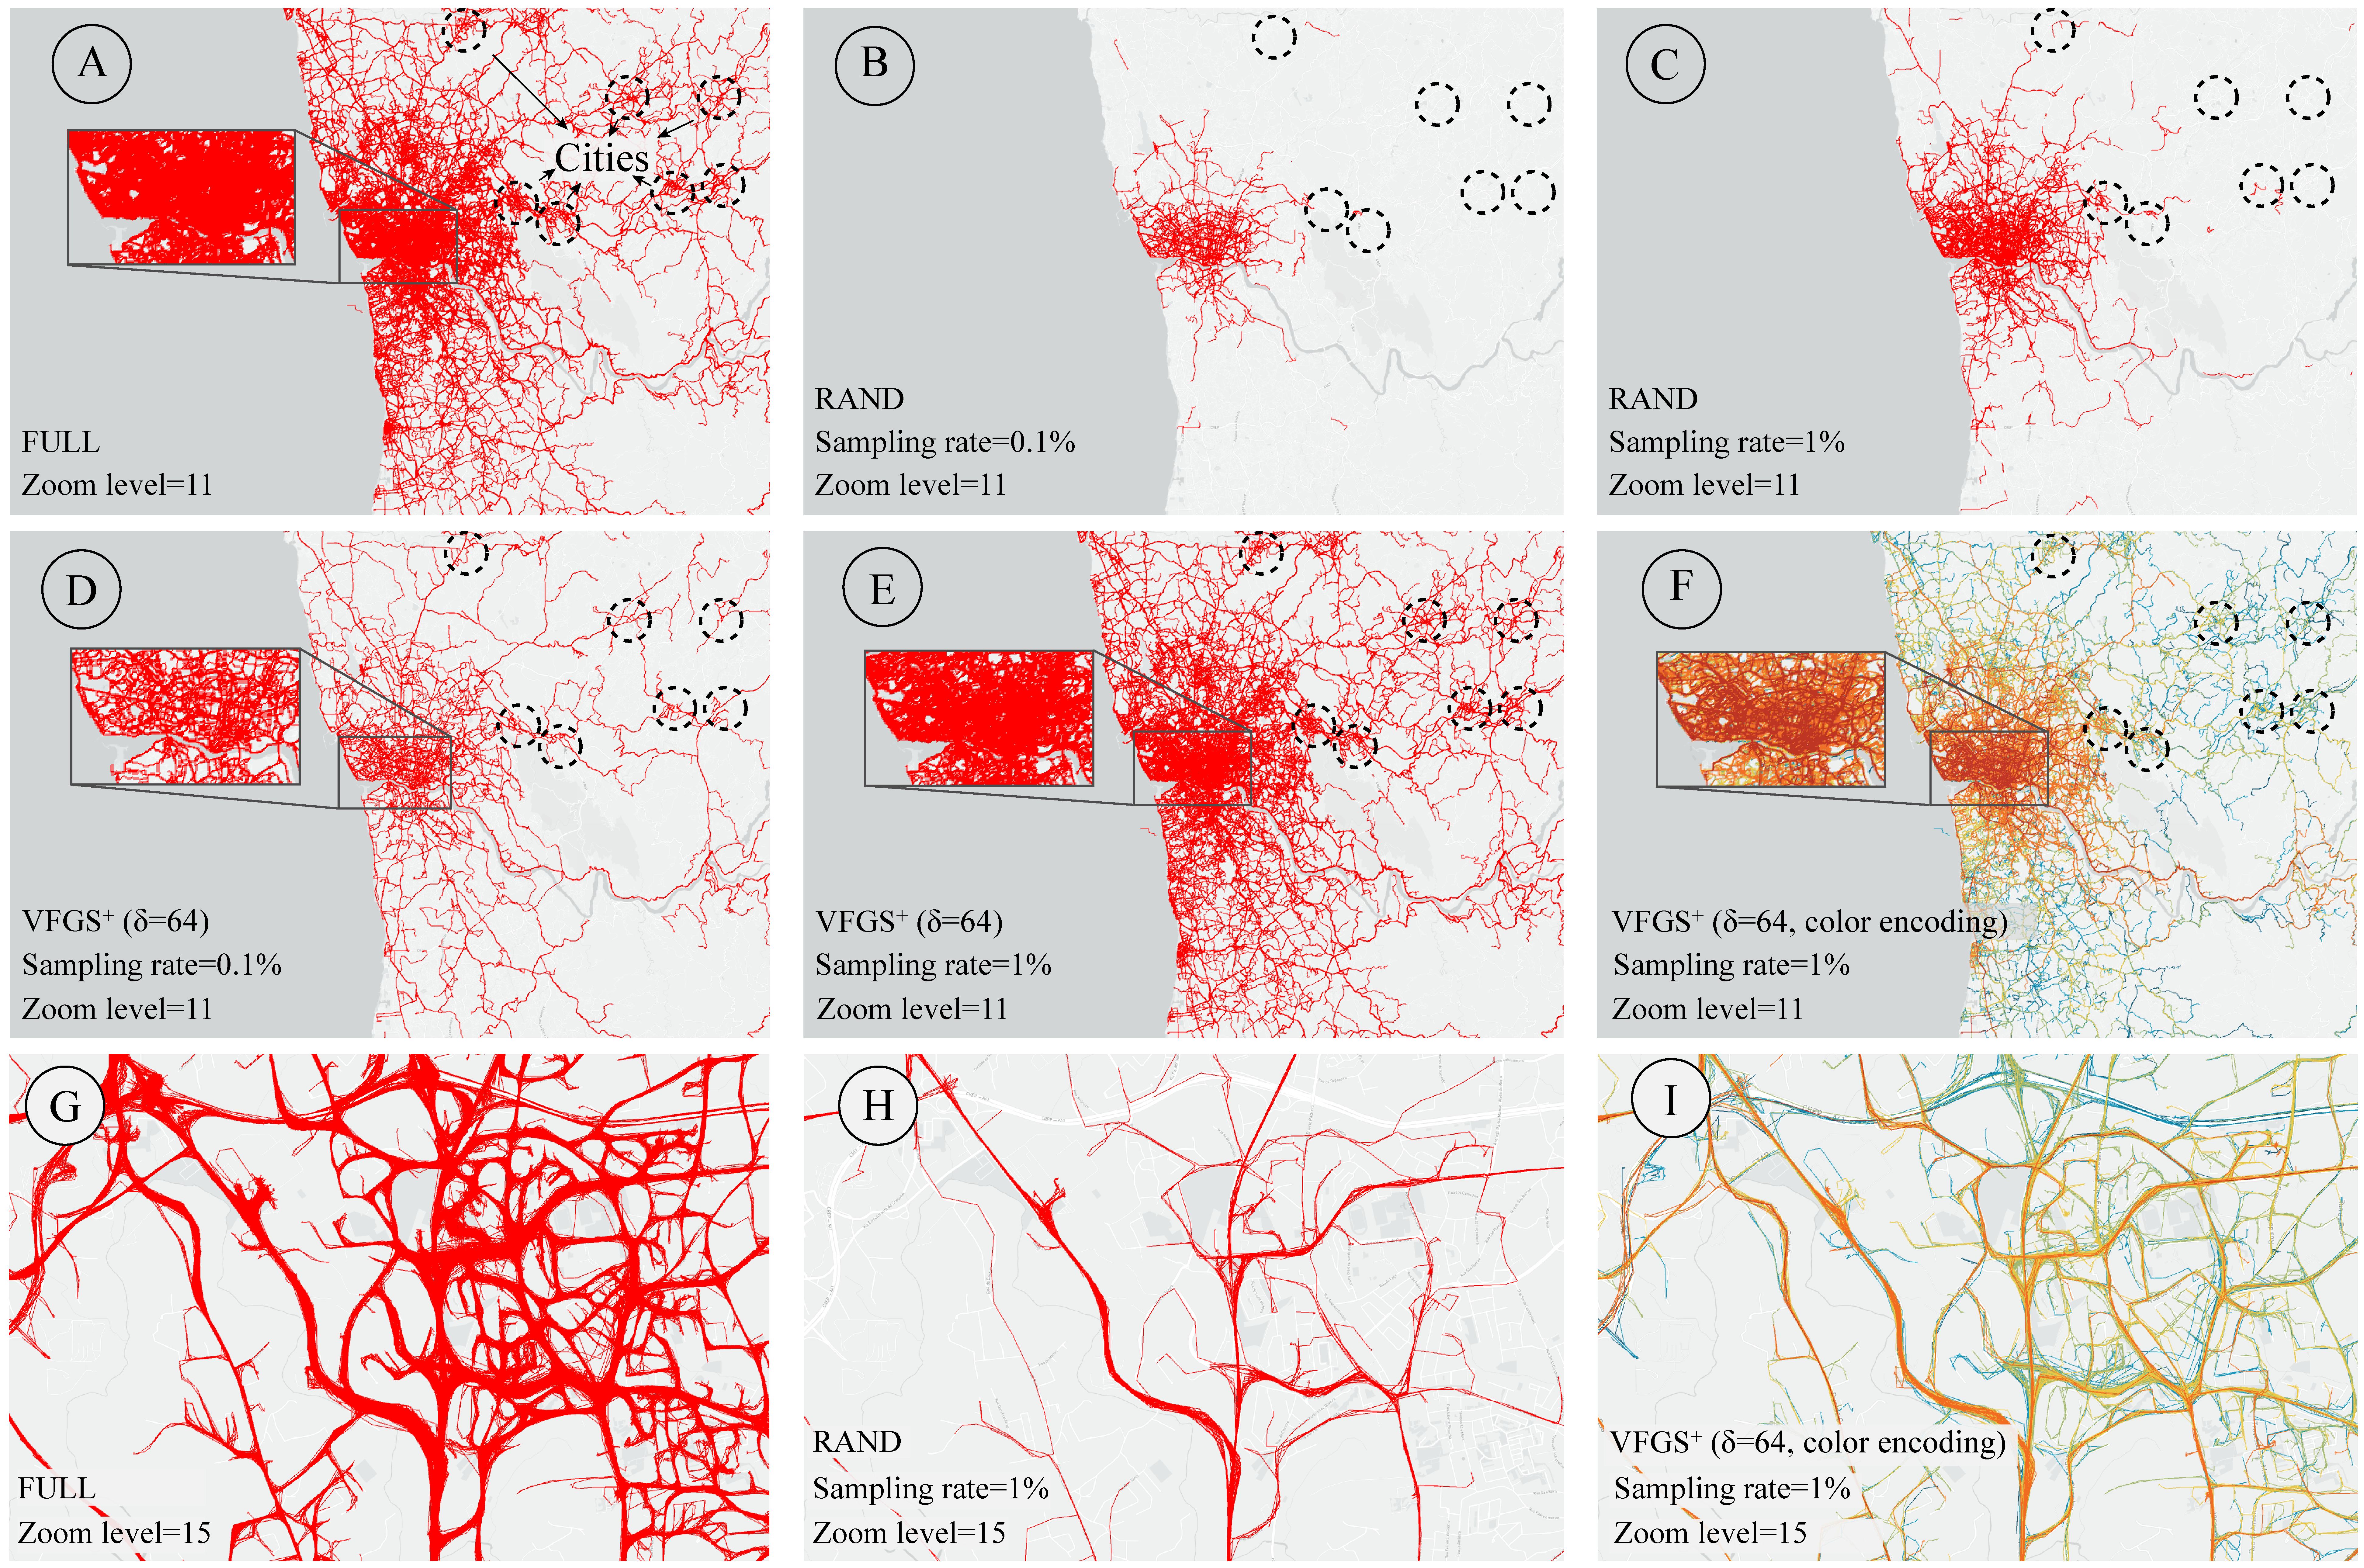
\includegraphics[width=0.90\textwidth]{pictures/Teaser.pdf}
% 	\vspace{-2mm}
% 	\caption{A comparison of visualization results. (I) A is the visualization of the full \pt{} taxi trajectory dataset at zoom level 11.
%     At the same zoom level, B and C are produced by uniform random sampling,
%     while D, E, F are produced by our $\avats$ algorithm.
%     (II) G is the visualization of the full \pt{} dataset at zoom level 15, while H and I are the corresponding results of uniform random sampling and $\avats$, respectively.
%     (III) F and I are generated by $\avats$ with color encoding for representativeness to combat visual clutter.
%     Best viewed in color.}
% 	\label{fig:teaser}
% \trim \trim
% \end{figure*}

% \QM{Introduce the data to visualization time: database/file - memory - data transformation(GPS to screen position)- visualization}.

Sampling techniques are widely used for large-scale data analysis in both database and visualization communities to reduce the visual clutter and improve the scalability~\cite{qin2020making,DBLP:conf/sigmod/DingHCC016,DBLP:journals/pvldb/KimBPIMR15,park2016visualization}. By sampling a subset of records from the raw large-scale dataset, it helps to reduce the data to visualization time. One such example is ScalaR~\cite{battle2013dynamic}, which employs a reduction layer between the visualization layer and the data management layer. The reduction layer samples records \textit{uniformly at random} (denoted as $\rand$) when the query results are too large. 

\QM{There are three challenges to design appropriate sampling methods for interactive visualizations: C1) guarantee the visual quality, C2) can be generated efficiently to support the interactive exploration, C3) support different-level of details.} 
However, $\rand$ does not work well for large-scale trajectory data visualization as it cannot provide quality guarantee. Take Figure~\ref{fig:overview}(B) for example, they are the visualization results generated by $\rand$ on the \pt{} taxi trajectory dataset with sampling rate  $1\%$. Obviously, it is very different from the visualization of the full \pt{} dataset in Figure~\ref{fig:overview}(A), since the random sampling method is easily ignore the data patterns in the spare areas. Another basic idea of the data reduction is to iteratively remove the trajectories \QM{which have the least impact of the whole visualization}~\cite{borcan2012improving}. Thus impact of a trajectory can be evaluated by sum of the distance(DTW or Fréchet distance) to all other trajectories. As shown by Figure.~\ref{fig:overview}, the visualization generated $\baseline$ is much better than $Rand$ by preserve more trajectories in the sparse region, but the general structure is still missing because it cannot theoretically guarantee the visual quality. Moreover the pairwise distance calculation for large trajectory dataset is very time consuming, which always needs days of preprocessing for millions of trajectories. 

%VLDB
%Sampling techniques are widely used for large-scale data analysis in both database and visualization communities~\cite{qin2020making,DBLP:conf/sigmod/DingHCC016,DBLP:journals/pvldb/KimBPIMR15,park2016visualization}. By sampling a subset of records from the raw large-scale dataset, it helps to reduce the rendering latency on graphics devices for visualization. One such example is ScalaR~\cite{battle2013dynamic}, which employs a reduction layer between the visualization layer and the data management layer. The reduction layer samples records \textit{uniformly at random} (denoted as $\rand$) when the query results are too large. However, $\rand$ does not work well for large-scale trajectory data visualization as it cannot provide fidelity guarantee. Take Figure~\ref{fig:teaser}(B) and (C) for example, they are the visualization results generated by $\rand$ on the \pt{} taxi trajectory dataset with sampling rate $0.1\%$ and $1\%$, respectively. Obviously, both of them are very different from the visualization of the full \pt{} dataset in Figure~\ref{fig:teaser}(A).


In this work, we set out to design efficient sampling algorithms that provides visual quality guarantee for large-scale line-based trajectory visualization. This goal leads to three research problems: (i) \emph{how to measure the visual quality of one visualization result?}(ii) \emph{how to tackle the visual clutter problem in large trajectory visualization?} 
(iii) \emph{how to devise an efficient sampling algorithm that \QM{balances visual quality and clutter from multi-level of details?}}  
To address these problems, we first propose a novel pixel-based \textit{visual quality loss function} to formally measure the difference between two visualizations and show that it is NP-hard to select a sized-$k$ sample of the trajectories to minimize the visual quality loss function. Next, we devise an \textit{visual quality guaranteed algorithm}named $\vats$, which provides theoretical visual quality guarantee for the sampled results. Then, we \textit{explicitly tackle the visual clutter problem} by taking data distribution and human perception characteristics into consideration in an advance algorithm named $\avats$. Case studies shows $\avats$ performs very well in the visualization of overview. Last, we maintain a visual quality tree which indexes the trajectories for multi level of regions thus to provide the quality guaranteed trajectory subset for the detail views. 

%VLDB
%In this work, we set out to design efficient sampling algorithms that provides visual fidelity guarantee for line-based large-scale trajectory visualization. This goal leads to three research problems: (i) \emph{how to measure the visual fidelity of one visualization result?} (ii) \emph{how to devise an efficient sampling algorithm that provides  guaranteed visual fidelity?} (iii) \emph{how to tackle the visual clutter problem in large trajectory visualization?} To address these problems, we first propose a novel pixel-based \textit{visual fidelity loss function} to formally measure the difference between two visualizations. We then show that it is NP-hard to select a sized-$k$ sample of the trajectories to minimize the visual fidelity loss function. Next, we devise an \textit{efficient approximate algorithm }named $\vats$, which provides theoretical visual fidelity guarantee for the sampled results. Last, we \textit{explicitly tackle the visual clutter problem} by taking data distribution and human perception characteristics into consideration in an advance algorithm named $\avats$.

%In this work, we propose visual fidelity-guaranteed sampling approaches for the line-based trajectory visualization problem.
%The technical challenges of our proposal are
%(i) \emph{how to define visual fidelity of visualization result theoretically?}
%(ii) \emph{how to devise an efficient sampling algorithm which offers visual fidelity guarantee on the visualization result?}
%and (iii) \emph{how to overcome the visual clutter in large trajectory visualization?}
%Specifically, we first propose a novel pixel-based visual fidelity loss function between two visualization results formally.
%With the visual fidelity loss function, we then prove it is NP-hardness to select a sized-$k$ subset of trajectories which has the minimal visual fidelity loss.
%Next, we devise an approximate algorithm $\vats$ which returns a sized-$k$ subset of trajectories and offers theoretical visual fidelity guarantee on the returning result.
%Last, we address the visual clutter issue explicitly by taking data distribution and human perception capability into consideration in the advance approach $\avats$.

\begin{figure*}[t]
	\centering
	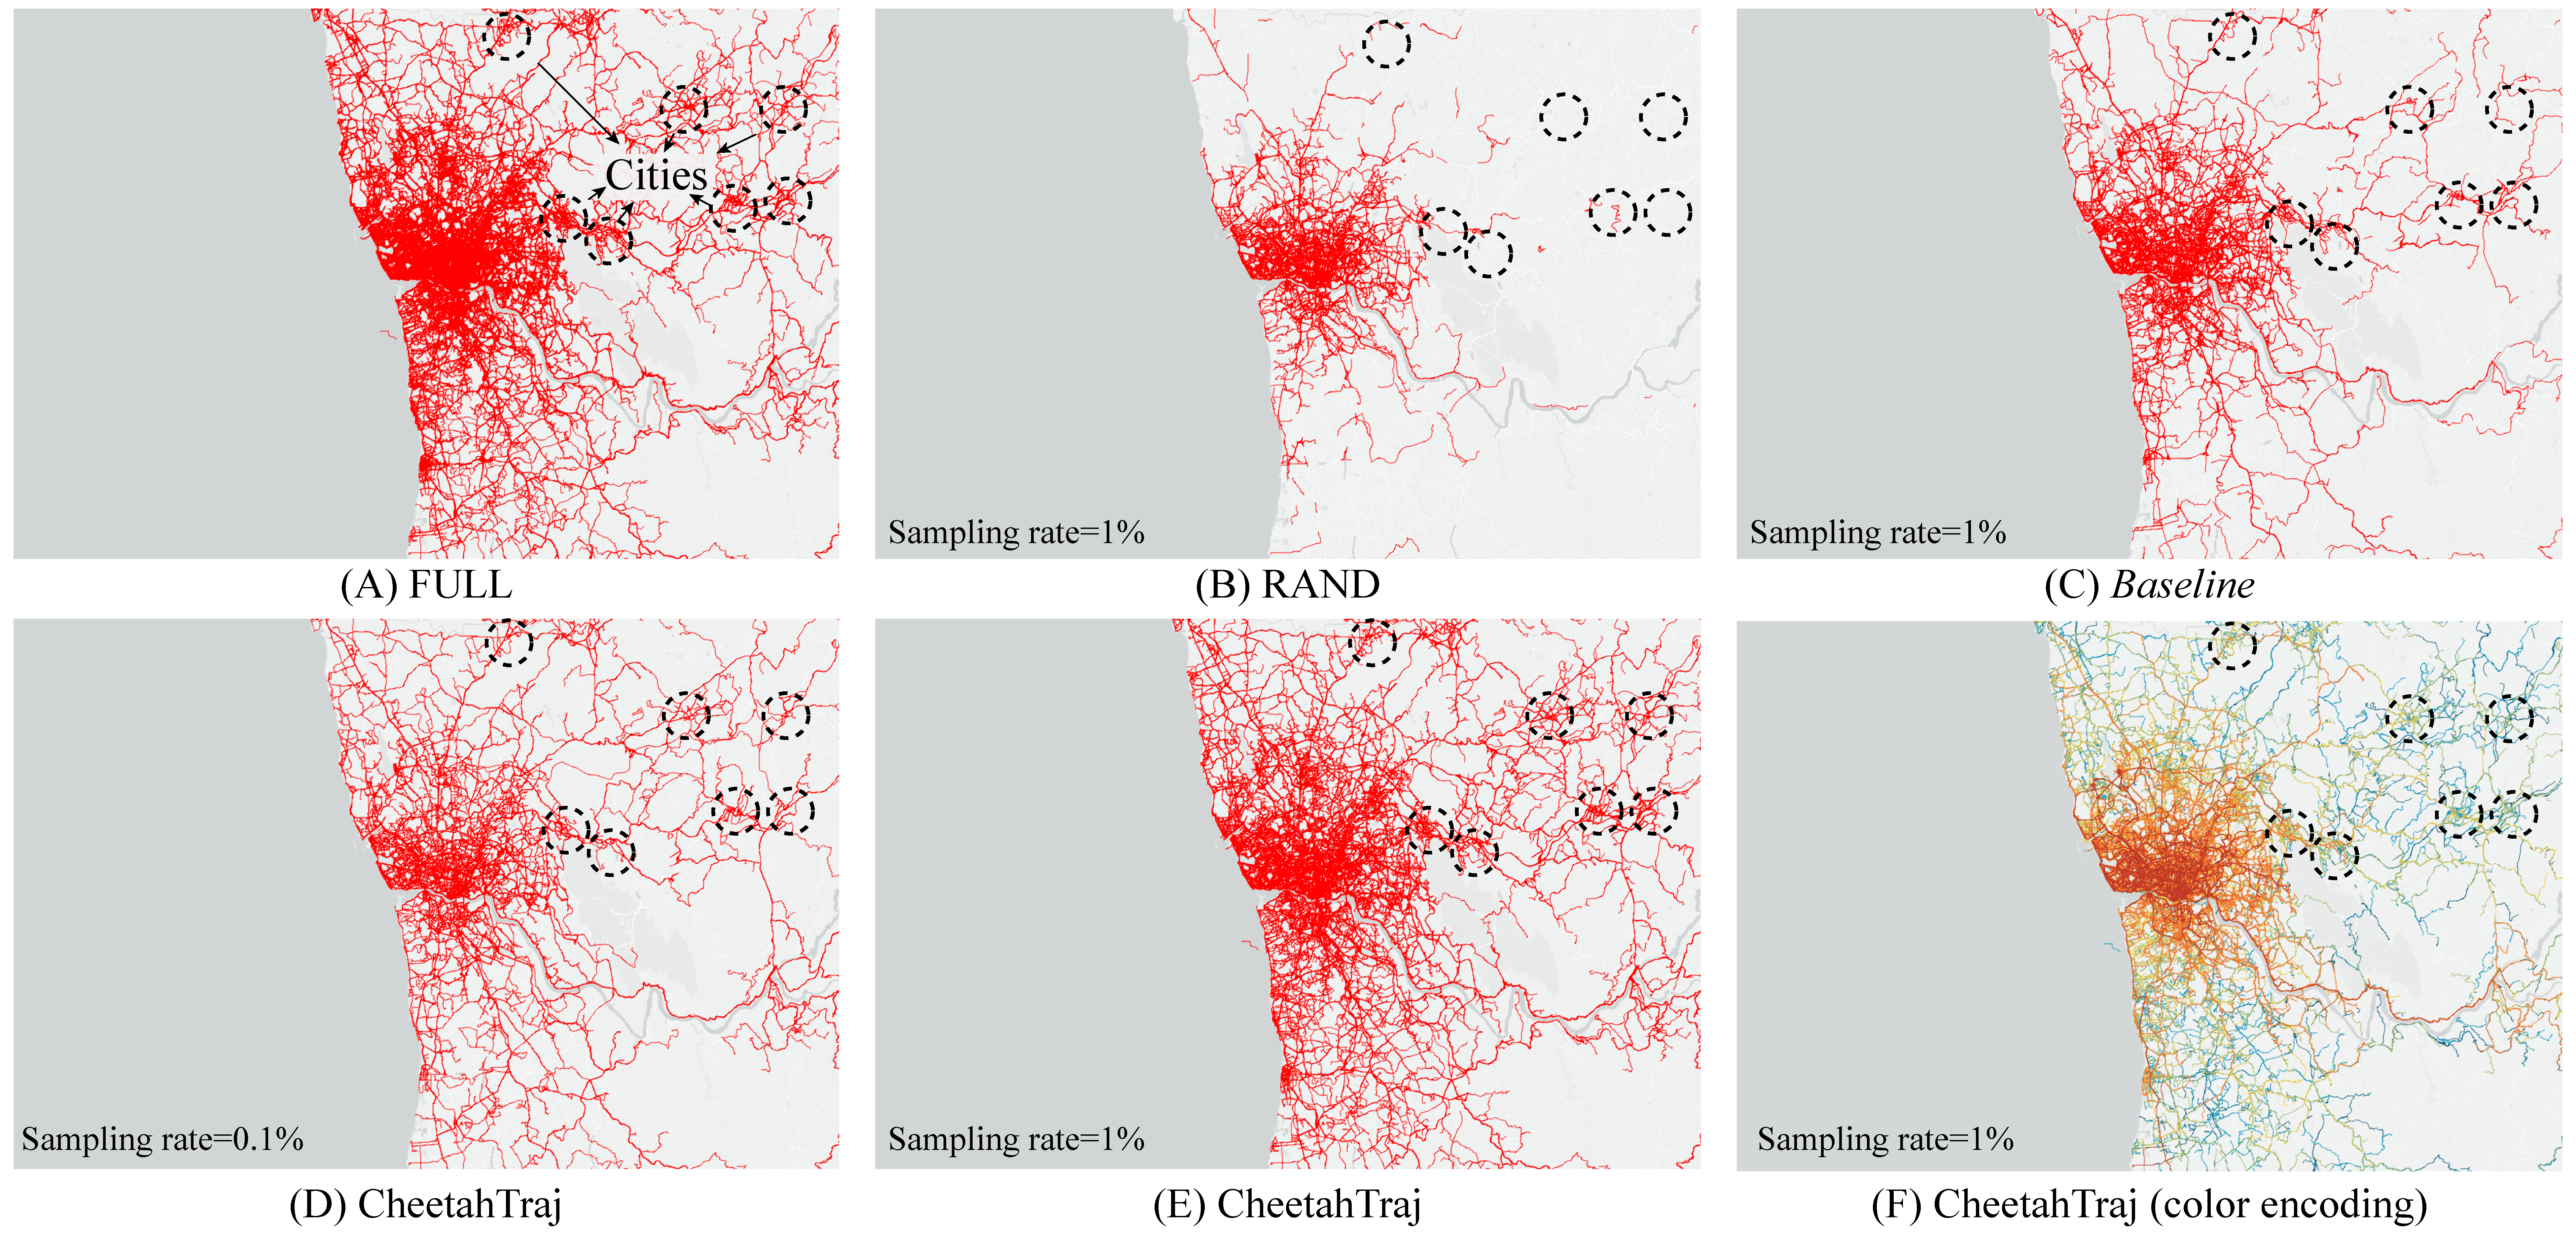
\includegraphics[width=0.95\textwidth]{pictures/case_study_icde/case_study_overview.pdf}
	\vspace{-3mm}
	\caption{Effectiveness of $\avats$ at overview visualization in \pt{}.}
	\label{fig:overview}
	\vspace{-2mm}
\end{figure*}


We illustrates the merits of our proposals in Figure~\ref{fig:overview}. Figure~\ref{fig:overview}(D) and (E) are the results of our $\avats{}$ algorithm on the \pt{} dataset with sampling rate $0.1\%$ and $1\%$, respectively. Compared with the uniform random sampling (i.e., $\rand$) and distance based sampling(i.e., $\baseline$) counterparts Figure~\ref{fig:overview}(B) and (C), they are obviously more similar to the full dataset visualization in Figure~\ref{fig:overview}(A). 
Further more, we colored the trajectories shown as Figure~\ref{fig:overview}(F) which is produced by our $\avats{}$ algorithm using the same parameters as Figure~\ref{fig:overview}(E) but the trajectories are colored according to their algorithm-generated representativeness (warmer color means more representative), thus the trajectory distribution information in the dense region can be easily observed.
% The advantage of our proposals over $\rand$ is also consistent across different zoom levels, e.g., Figure~\ref{fig:overview}(E) vs. Figure~\ref{fig:overview}(C) at level 11, and Figure~\ref{fig:overview}(I) vs. Figure~\ref{fig:overview}(H) at level 15. Figure~\ref{fig:overview}(F) is produced by our $\avats{}$ algorithm using the same parameters as Figure~\ref{fig:overview}(E) but the trajectories are colored according to their algorithm-generated representativeness (warmer color means more representative). Observe that the visual clutter problem in Figures~\ref{fig:overview}(A) and (E) are significantly alleviated in Figure~\ref{fig:overview}(F) with color encoding. This advantage is even more prominent when comparing Figure (I) with Figure (G) and (H).




%Figures~\ref{fig:teaser}(D) and (E) show the visualization results of our proposal $\avats{}$ on \pt{} taxi trajectory dataset with {the} sampling rate $0.1\%$ and $1\%$, respectively.
%Comparing with the corresponding visualization results of uniform random sampling method $\rand$ in Figure~\ref{fig:teaser}(B) and (C),
%the superiority of $\avats$ is obvious.
%% Obviously, the visualization fidelity of them are much better than the uniform random sampling visualization results with the same sampling rates, see Figure~\ref{fig:teaser}(B) and (C).
%Figures~\ref{fig:teaser}(F) is the returning result of our proposal, which colors the trajectories {according to the trajectory representativeness}.
%It has the same parameters of Figure~\ref{fig:teaser}(E).
%Visually, the visual clutter issue in Figures~\ref{fig:teaser}(A) and (E) are alleviated in Figure~\ref{fig:teaser}(F).
%In addition, our proposals are robustness with different zoom levels.
%%Figure~\ref{fig:teaser}(G), (H), and (I) depict the visualization results of the \pt{} dataset, the returning result of uniform random sampling $\rand$ and the returning result of $\avats$ with color encoding at zoom-level 15, for example, we can obtain them by zooming in the visualization result in Figure~\ref{fig:teaser}(A), (C), and (F), respectively.
%Consider the visualization results in Figures~\ref{fig:teaser}(G), (H), and (I) with zoom level 15.
%Intuitively, the visualization result of our proposal $\avats$ in Figure~\ref{fig:teaser}(F) outperforms the uniform random sampling $\rand$ in Figure~\ref{fig:teaser}(H) significantly.
%It even performs better than Figure~\ref{fig:teaser}(G), the visualized result of the \pt{} dataset, as it reduces visual clutter in Figure~\ref{fig:teaser}(G) by using color encoding scheme to capture the representativeness of different trajectories.

To sum up, our contributions in this paper include:
%\setlist{nolistsep}
%\begin{itemize}[noitemsep]
\squishlist
  \item We formulate the visual quality-guaranteed sampling problem for large-scale trajectory data visualization, and prove that it is {NP-hard} in Section~\ref{sec:pro}.
  \item We devise an approximate algorithm $\vats$ for the visual quality-guaranteed sampling problem with a suite of efficiency optimizations including submodularity and lazy computation in Section~\ref{sec:sol}.
  \item We propose an advance algorithm $\avats$ to tackle the visual clutter problem by introducing a perception tolerance parameter, and encoding the representativeness of trajectories using different colors in Section~\ref{sec:aa}.
  \item We propose an advance algorithm $\avats$ to tackle the visual clutter problem by introducing a perception tolerance parameter, and encoding the representativeness of trajectories using different colors in Section~\ref{sec:aa}.
  \item We conduct extensive experiments on real-world trajectory datasets to demonstrate the superiority of our proposals in Section~\ref{sec:exp}. In particular, nearly 200 real users are recruited to test the effectiveness of our methods on three practical applications.
\squishend
%\end{itemize}

% in Section~\ref{sec:pro}

%Our proposal demonstrates their superiority over existing methods
%With the same sampling set size($1\%$), the proposed method generates a higher-fidelity visualization and .

%With the loss function, we analyze the hardness of the problem, and devise a visual quality guaranteed sampling algorithm for it.
%Figure~\ref{fig:compare} depicts an comparison among the ground truth,  uniform random sampling and our proposed method.
%With the same sampling set size($1\%$), the proposed method generates a higher-fidelity visualization and support the multi-resolution very well.
%At last, color encoding are applied to enhance the distribution of trajectories.

%


%\TB{Visualizing a large collection of trajectories are used frequently in map service or smart city applications.}
%The most popular and conventional method is the line-based visualization~\cite{chen2015survey}: connecting the passing points of movement objects by polylines.
%To handle the big dataset, many visualization products such as Spotfire~\footnote{\url{https://www.tibco.com/products/tibco-spotfire}}
%and Tableau~\footnote{\url{https://www.tableau.com/}} support advanced database management systems as a ``backend'' for the efficient data processing the query.
%The current visualization tools always don't scale well for the presentation of very large trajectory dataset due to the two challenges,
%visual clutter and limited rendering speed, which hinders the abilities of human-users for interactively exploring the dataset and identifying the movement patterns.
%In recent years, most of the visualization research works mainly try to address the visual clutter issue by proposing new techniques such as the
%spatial aggregation~\cite{zeng2013visualizing, von2015mobilitygraphs}, edge bundling~\cite{zeng2019route, thony2015vector} and density map~\cite{lampe2011interactive, scheepens2011interactive}.
%Instead, in this paper, we focus on the challenge of inefficient rendering in the large trajectory dataset by involving data sampling techniques.

%It is time consuming to generate very simple visualization when the data size become very large. Using Porto taxi data ~\footnote{\url{http://www.geolink.pt/ecmlpkdd2015-challenge/dataset.html}} as an example, Table~\ref{table:rendering_time} demonstrates the rendering time at each dataset size. \ZW{shall also mention which rendering toolkit is used here.} It shows that normal method takes more than 14 minutes (\ZW{seconds?}) to generate the graphics for 1 million trajectories, which is far beyond the human-acceptable response time for the interactive exploration~\cite{shneiderman1984response}.
%One work closely related to ours is ScalaR~\cite{battle2013dynamic}, which adds a reduction layer between visualization layer and data management layer. The reduction layer uses an uniform random sampling method to sample data once the query results are large enough, thus to reduce the amount of data to be visualized.
%Further more, Park et al. propose VAS~\cite{park2016visualization} which implements new sampling techniques to guarantee the visual quality.
%However, these sampling techniques are designed for the simple dataset, and have been approved effective in scatter plot or map plot.
%However, the trajectory sampling is more challenge due to the complexity of data form(e.g. varying lengths, lack of compact representation, difficulty in measuring the similarity) that makes traditional density-biased sampling techniques inappropriate.
%A naive solution to employ sampling idea for large-scale trajectory visualization problem is randomly selecting several trajectories from the data set then visualize it by graphics device.
%However, the visualization result may be not acceptable by the user because of the visual information loss in the sparse distributed regions.





%
%\begin{figure}[t]
%	\centering
%	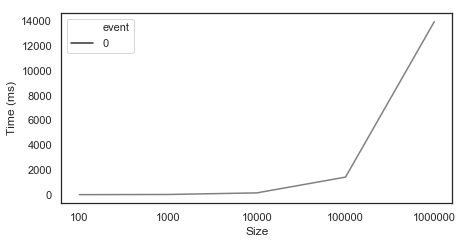
\includegraphics[width=0.4\textwidth]{pictures/introduction/timesize.png}
%	\vspace{-5mm}
%	\caption{The latency time for generating line-based visualization at each datasize.}
%	\vspace{-5mm}
%	\label{fig:rendering_time}
%\end{figure}




%The major challenges to design visual quality guaranteed sampling method are:
%(I) how to define visual quality theoretically? (II) how to guarantee the quality of the sampling-based visualization result?
%\TB{In this work, we study how to reduce the rendering time and preserve the visual quality for the large-scale trajectory visualization.}
%We extend the motivation of visualization-aware sampling to trajectory dataset and propose a novel sampling strategy, \textbf{v}isualization \textbf{a}ware \textbf{t}rajectory \textbf{s}ampling(VATS), that produces high-visual-quality line-based trajectory visualization at different zooming resolutions.
%%\QM{In this paper, we first proposed the visual fidelity loss function which effectively evaluates the visual loss of the sampling method. Then we minimize the loss function by transforming this problem to an optimization problem. Several solutions for efficiently solving the optimization problem are discussed.}
%We first format visual quality by defining the loss function between the visualization results of the whole dataset and sampled dataset.
%With the loss function, we analyze the hardness of the problem, and devise a visual quality guaranteed sampling algorithm for it.
%Figure~\ref{fig:compare} depicts an comparison among the ground truth,  uniform random sampling and our proposed method.
%With the same sampling set size($1\%$), the proposed method generates a higher-fidelity visualization and support the multi-resolution very well.
%At last, color encoding are applied to enhance the distribution of trajectories.
%
%\begin{figure}[t]
%	\centering
%	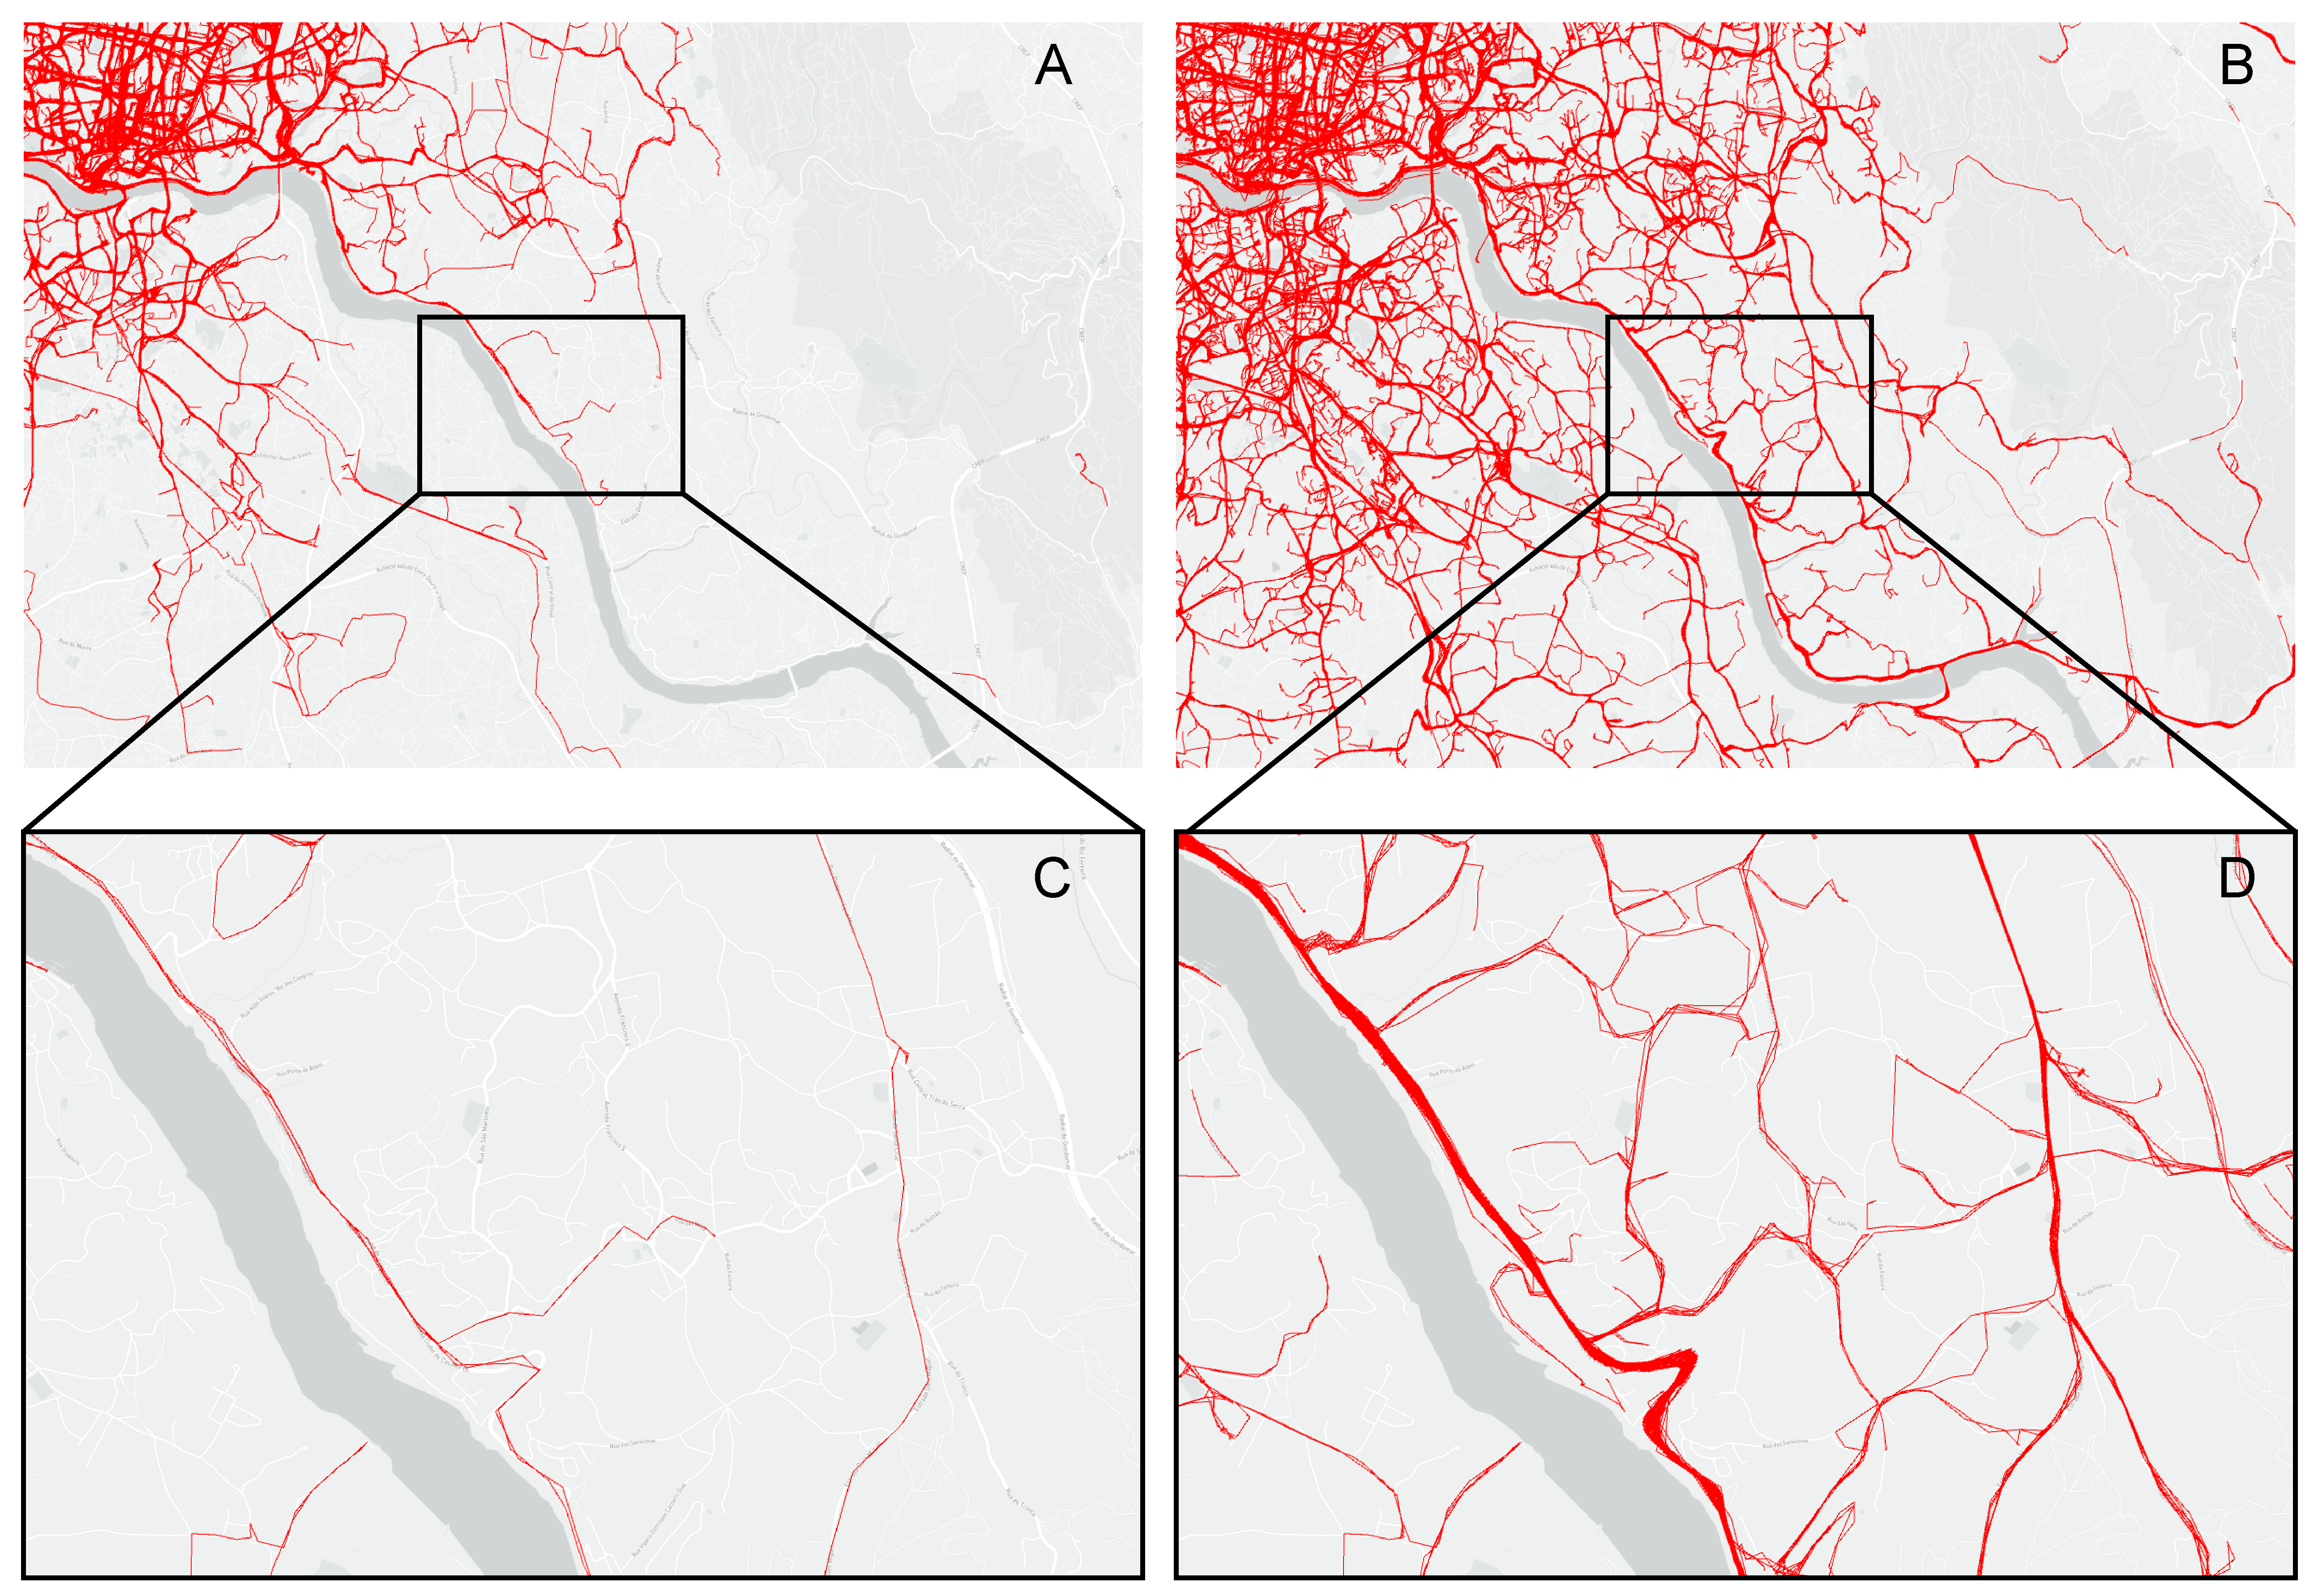
\includegraphics[width=0.44\textwidth]{pictures/introduction/effectiveness.pdf}
%	\vspace{-3mm}
%	\caption{Trajectory sampling generated by uniform random sampling(A,C) and VQGTS(B,D) at same sampling rate. In both high-level(A,B) and low level(C,D) view, our approach preserved more detail information about the trajectories especially for the sparse regions.}
%	\vspace{-5mm}
%	\label{fig:compare}
%\end{figure}
%

%
% \Bo{we can keep it at technical report.}
%The remainder of this paper is organized as follows. Section~\ref{sec:rel} discusses the related work, and Section~\ref{sec:pro} formally formulates our problem and analyze its hardness. Section~\ref{sec:sol} presents our approximate solution for the problem along with the optimization techniques. The advanced solution for visual clutter is introduced in Section~\ref{sec:aa}. Section~\ref{sec:exp} elaborates the extensive experimental studies. Section~\ref{sec:con} concludes this paper and highlights possible future directions.


%Section~\ref{sec:pro} formulates our problem and analyze its hardness.
%Section~\ref{sec:sol} provides an approximate solution for it, together with a suite of optimization techniques.
%Section~\ref{sec:aa} proposes an advanced solution for our problem.
%Section~\ref{sec:exp} elaborates our extensive experimental studies and our findings in detail.
%Section~\ref{sec:con} concludes this work and highlights the promising future directions.



\section{Related work}\label{sec:rel}
%In this section, we survey previous work and focus on the most relevant pieces.
%Section~\ref{sec:trajvisana} and ~\ref{sec:interactive} summarize the related works in trajectory visual analysis and interactive data visualization for large dataset, respectively.

In this part, we survey related works on \textit{trajectory visualization methods} in Section~\ref{sec:trajvisana} and \textit{interactive data visualization for large datasets} in Section~\ref{sec:interactive}, respectively.

\subsection{Trajectory Visualization Methods}\label{sec:trajvisana}
A trajectory is a sequence of spatial locations (e.g., GPS positioning results) and trajectory is the most common representation of object movements. Existing trajectory visualization methods can be classified into three categories according to the form of visualization~\cite{chen2015survey}, i.e., \textit{point-based visualization}, \textit{region-based visualization}, and \textit{line-based visualization}. We give a brief introduction to these methods and refer the interested readers to~\cite{chen2015survey} for more detailed discussions. Point-based visualization plots the locations in each trajectory independently and captures the overall spatial distribution of the moving objects. Many density-based methods, e.g., kernel density estimation, are applied in point-based visualization~\cite{liu2013vait,yang2016exploring,chae2014public,xie2008kernel, borruso2008network} to preserve the spatial distribution. Region-based visualization slices the entire region into sub-regions and visualizes the aggregated information in each sub-region~\cite{guo2009flow,wood2010visualisation,von2015mobilitygraphs}. As region-based visualization focuses on aggregated statistics, it is effective in capturing macro-patterns. In this work, we focus on line-based visualization, which uses polylines to connect the locations in each trajectory and shows the trace of object movements (see examples in Figure~\ref{fig:line}). As it preserves the continuous movement information of objects~\cite{guo2011tripvista,hurter2009fromdady}, line-based visualization is widely used in many visual analysis applications such as traffic management, urban planning, and route recommendation. However, line-based visualization is known to suffer from serve visual clutter, especially when the dataset is large. Several techniques have been proposed to alleviate visual clutter, such as clustering-based techniques~\cite{ferreira2013vector, rinzivillo2008visually, von2015mobilitygraphs} and advanced interaction techniques~\cite{kruger2013trajectorylenses, ferreira2013visual}.



\subsection{Interactive Visualization for Large Datasets}\label{sec:interactive}
%With the recent advancement of location-acquisition technology, the size of available trajectory dataset becomes extremely huge.
%For example, the operating taxis in Shenzhen generate {$\sim$}9.3GB trajectory data per day.
%Figure~\ref{fig:framework} illustrates the architecture of interactive visualization systems for large datasets,
%e.g., Spotfire~\cite{Spotfire}, Tableau~\cite{Tableau}, ATLAS~\cite{chan2008maintaining}, and Viate~\cite{yang2019vaite}.
%{It} consists of three layers: the user interface in front-end, the optimization techniques in middle-layer, and the (cloud-based) database management system in the back-end.
%{Typically, the researchers in visualization community focus on improving the effectiveness of data visualization at the front-end,
%e.g., designing novel visualization method D3~\cite{d3} to assist data analysts to obtain data insights effectively.}
%For the researchers in database community, they are working on the efficiency aspect for large data processing,
%e.g., devising big data processing system Spark~\cite{spark} for efficient query processing at back-end.
%In recent years, both visualization and database communities are dedicating to advance the techniques in interactive visual analysis for large-scale dataset,
%e.g., the optimizations in the middle-layer (see Figure~\ref{fig:framework}).
%We briefly elaborate these optimization techniques {in this section}.






Figure~\ref{fig:framework} illustrates the general architecture of interactive visualization systems,
e.g., Spotfire~\cite{Spotfire}, Tableau~\cite{Tableau}, ATLAS~\cite{chan2008maintaining}, and Viate~\cite{yang2019vaite}.
There are typically three layers: user interface in the front-end layer, optimization techniques in the middle-layer, and database management system (usually cloud-based) in the back-end layer. Researchers in the visualization community usually focus on improving the effectiveness of data visualization at the front-end, e.g., designing novel visualization methods/toolkits such as D3~\cite{d3} to enable data analysts to gain insights from data effectively. For researchers in the database community, they usually aim to improve query efficiency, e.g., devising big data processing systems such as Spark~\cite{spark} for efficient data processing at the back-end. With recent developments of location-acquisition technologies, the sizes of available trajectory datasets have become extremely large. For example, the operating taxis in Shenzhen generate {$\sim$}9.3GB trajectory data per day. However, large datasets increase visualization generation latency due to heavy data processing/graphic rendering, which harms the responsiveness of interactive visualization. Therefore, both visualization and database communities began to advance techniques in the middle-layer to reduce the visualization latency for large datasets. We briefly elaborate these techniques as follows.


\begin{figure}
	\centering
	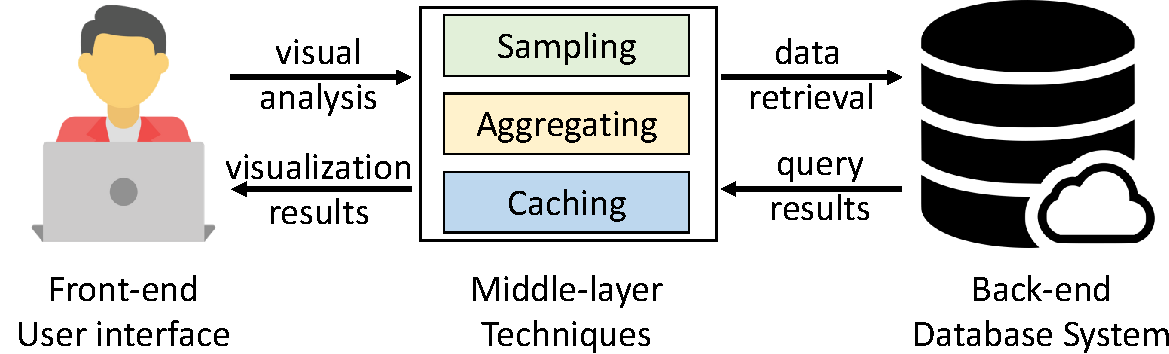
\includegraphics[width=0.40\textwidth]{pictures/framework/framework.pdf}
	\vspace{-2mm}
	\caption{System architecture for interactive visualization.} \label{fig:framework}
    \vspace{-2mm}
\end{figure}


\stitle{Aggregating-based techniques}
%{Aggregating-based techniques pre-process raw data with aggregation techniques (e.g., clustering) in the middle-layer, and yield fewer rendering objects for interactive visual analysis.}
%Returning to the trajectory visual analysis,
These works~\cite{wood2010visualisation,guo2009flow,von2015mobilitygraphs} divide the {spatial space} into basic units and visualize the aggregated information of the trajectories for each unit. For more details on aggregating-based techniques, we refer the reader to the related works~\cite{andrienko2008spatio,adrienko2010spatial}. Our problem and solutions are different from these works as we focus on visualizing the raw input data, instead of the aggregated results.
%However, aggregating-based methods will cause information loss definitely.
%For instance, the continuous spatial traces of the moving objects are always missing and the rarely appeared trajectories are easily to be ignored.






\stitle{Sampling-based techniques}
Sampling techniques are widely used in both visualization and database communities ~\cite{battle2013dynamic,chen2014visual,park2016visualization,qin2020making,DBLP:conf/sigmod/DingHCC016,DBLP:journals/pvldb/KimBPIMR15}.
%are well-studied in the interactive visualization problems with large-scale input data.
%It is
%In particular, ~\cite{chen2014visual} devised a sampling algorithm to preserve the meaningful data items.
% according to the analyzing requirement such as the multi-class data analysis and hierarchical exploration.
The work most relevant to ours is~\cite{park2016visualization}, which is designed for scatter plots (a form of point-based visualization). It solves the problem of point overdrawing and preserves the spatial point distribution of the original dataset at the same time. The techniques in~\cite{park2016visualization} cannot be adapted to our trajectory visualization problem
as trajectory is more complex than scatter points (e.g., varying lengths, contiguous GPS points).
%(i) the complexity of the trajectories~\cite{pelekis2010unsupervised}, and (ii) the loss function and its corresponding solutions are specified for scatter plot, not applicable for line-based trajectory visualization.
%For trajectory visual analysis,  most of the existing trajectory sampling techniques (if not all) cluster the trajectories at first,
%then select the most representative trajectories from each cluster and visualize them.
%It is impractical to provide interactive visualizations for real-world applications as
%trajectory clustering is still an open problem in both database and visualization communities~\cite{panagiotakis2011segmentation,agarwal2018subtrajectory}.

%as
%(i) the trajectory similarity computation and clustering algorithms are very expensive~\cite{pelekis2007similarity},
%and (ii) the



\stitle{Caching-based and other techniques}
%Caching is commonly used to improve the performance of large data processing system, e.g., search engine~\cite{xu2015diversified}.
Chan et al. present ATLAS~\cite{chan2008maintaining}, which utilizes caching for efficient data communication between server and client.
In addition, ATLAS also exploits a powerful multi-core server to accelerate visual analysis task processing from the middle-layer to the back-end.
Piringer et al.~\cite{piringer2009multi} propose a multi-threading architecture for interactive visual exploration,
which utilizes multi-core devices and avoids the pitfalls of multi-threading to provide quick visual feedback.
{Our} techniques in this work are orthogonal to researches in this category.

%Current advancing sampling techniques in the visualization domain are mostly
%Some works design advanced sampling algorithms to preserve the meaningful data items according to the analyzing requirement such as the multi-class data analysis and hierarchical exploration~\cite{chen2014visual}. Furthermore, to the usage of more visual channels of the points other than location such as color~\cite{chen2014visual}, size~\cite{woodruff1998constant} and opacity are discussed.
%Closely related to our work, Park et al.~\cite{park2016visualization} proposed the visualization-aware techniques for the scatter plot.
%
%In comparison with the sampling techniques for scatter plot, the trajectory sampling is more challenging because of the complexity of the trajectories~\cite{pelekis2010unsupervised}.
%
%
%Many exiting visual analytics systems leverage powerful database manage system as the backend to facilitate the fast data processing. Based on the solution proposed in ScalaR~\cite{battle2013dynamic}, a common visualization framework involving sampling technique is illustrated as Figure~\ref{fig:framework}, where a sampling layer is set between the backend and frontend. Since the sampling methods are always designed for complicated task, the algorithms may not be efficient enough to support the interactive data exploration. Thus the cache model is always implemented to save the sampling results. In our scenario, the users query large amount of data(e.g. all Shenzhen trajectories in one week) once and then conduct interactive multi-resolution exploration based on the sampled data, thus the method need to guarantee the visual quality well across different resolutions.
%
%Sampling is a delta-facto solution for the problems with big data. Target at the sampling requirement, the naive solutions such as uniform random sampling cannot generate acceptable because the serious visual information loss. In this section, we first define a loss function to evaluate the visual quality between the visualization results between whole dataset and sampled subset. Then we analyze the hardness of the problem and design algorithms for it.
%
%
%\begin{figure}[t]
%	\centering
%	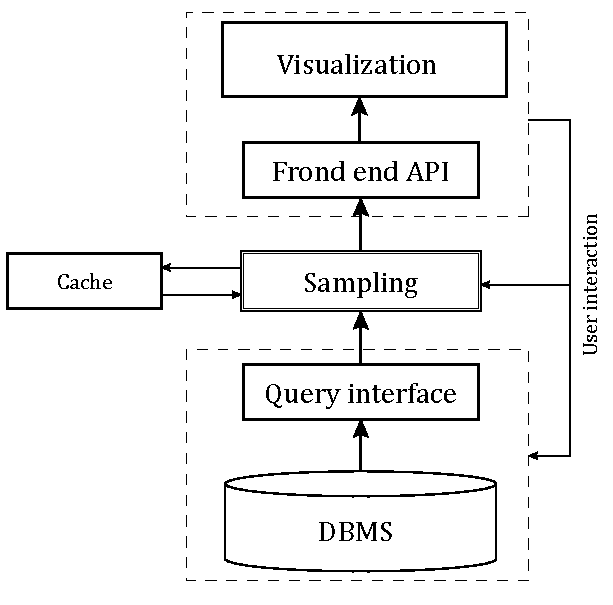
\includegraphics[width=0.3\textwidth]{pictures/framework/DBVAframework.pdf}
%	\vspace{-5mm}
%	\caption{A visualization framework involving sampling layer between the front-end and database management system.}
%	\vspace{-5mm}
%	\label{fig:framework}
%\end{figure}
%

\sstitle{Novelties of our work} To the best of our knowledge, we are the first to observe that random sampling harms visual fidelity for large-scale trajectory visualization and formulate the problem of fidelity-guaranteed sampling. To tackle this problem, we design a complete framework with fidelity loss function, theoretical fidelity loss analysis, and algorithm efficiency optimizations. The well-know visual clutter problem of trajectory visualization is also addressed naturally in our sampling framework. Extensive experimental results show that our proposals effectively maintain visual fidelity and reduces visualization latency at the same time.


%Our work differs from the above researches as we propose visual fidelity-guaranteed sampling approaches for the large-scale trajectory visualization problem,
%we demonstrate the superiority of our proposals by case-, user- and quantitative- studies in real-world dataset.
%
%Unlike existing line-based visualization techniques, we propose visual fidelity-guaranteed sampling approaches for line-based trajectory visualization with large-scale input data.
%To the best of our knowledge, it is the first work which offers theoretical visual fidelity guarantee on the sampling result for large-scale line-based trajectory visualization. 

\section{Problem Formulation}\label{sec:pro}
In this part, we first formally define the \textit{fidelity-optimal sampling problem} in Section~\ref{sec:def} and then show that it is NP-hard to solve the problem exactly in Section~\ref{sec:hard}.

\begin{figure}
	\centering
	\small
	\begin{tabular}{cc}
        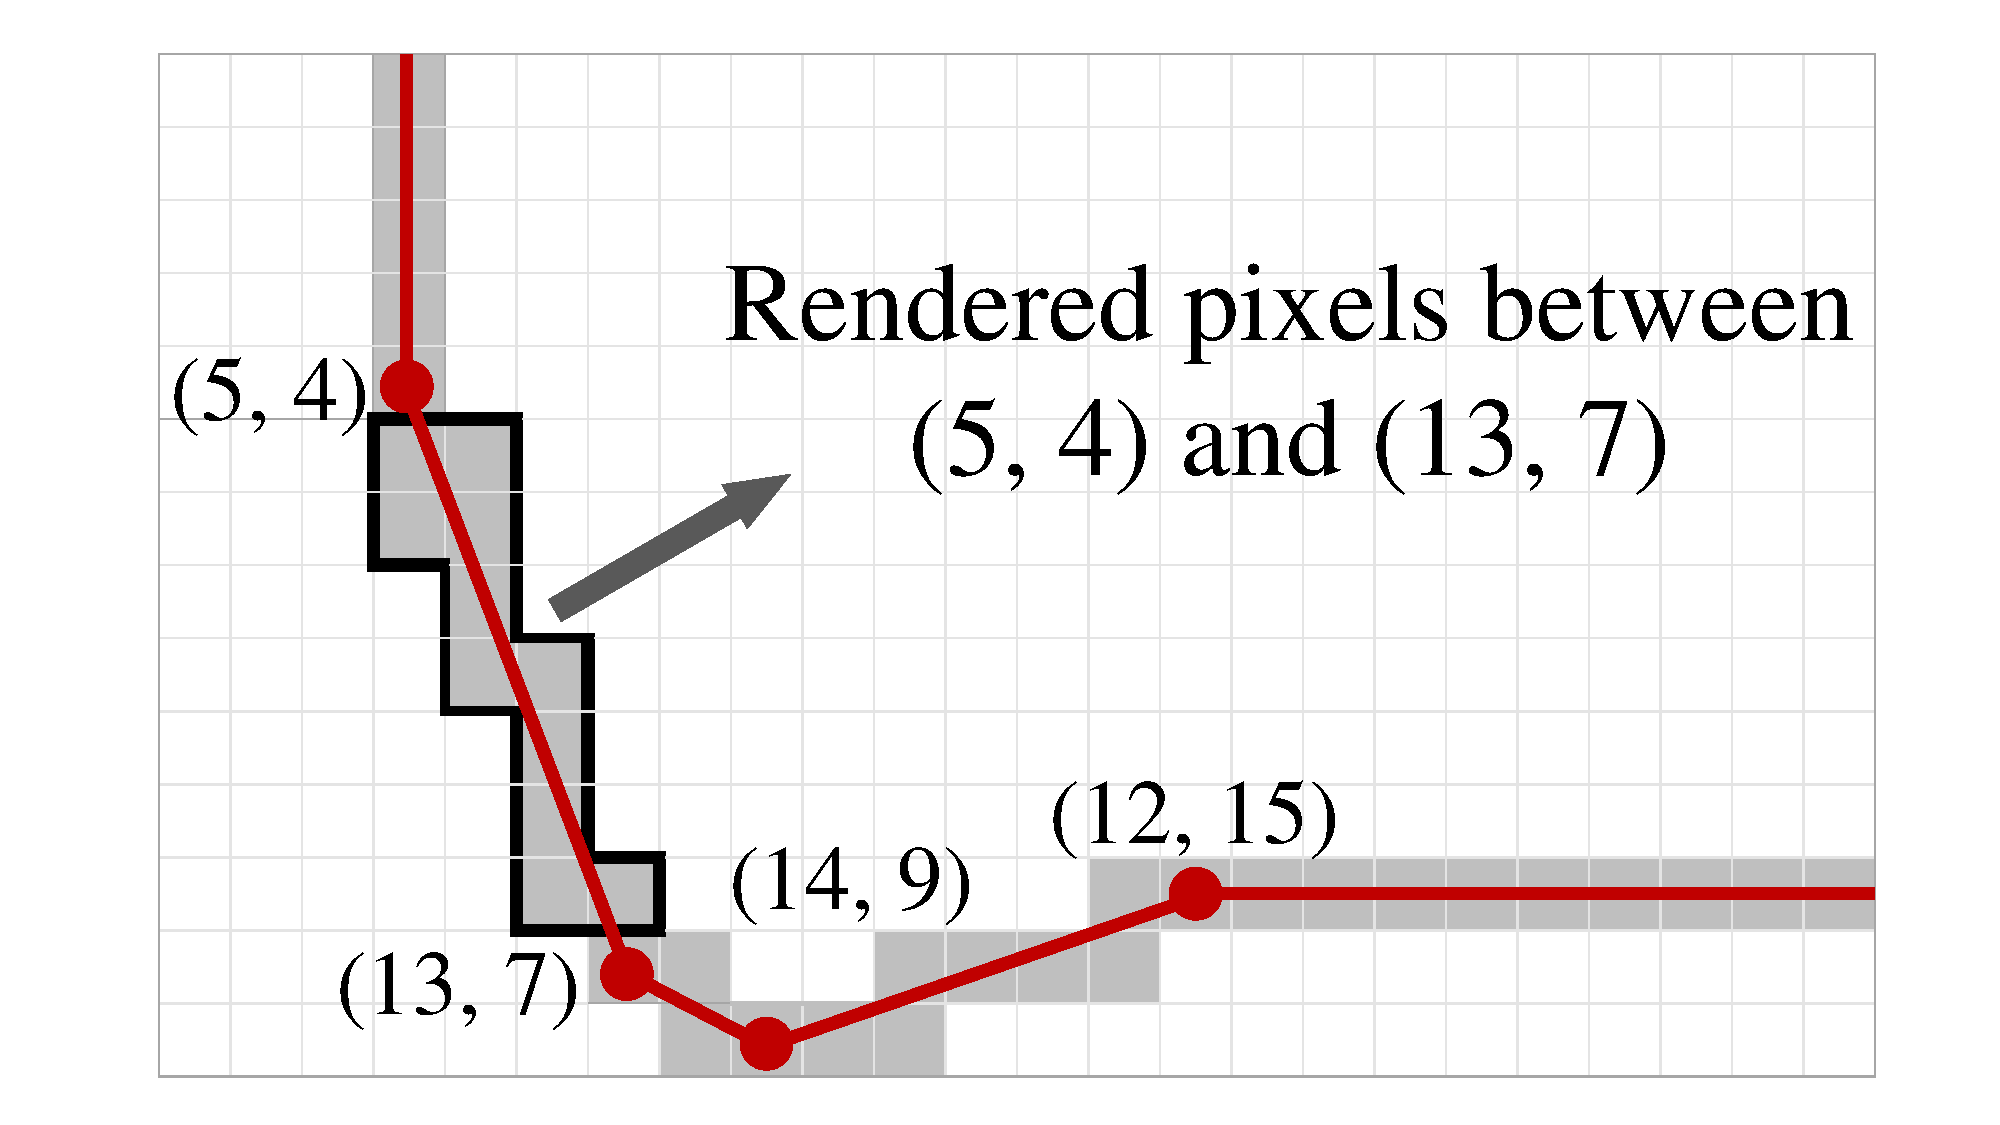
\includegraphics[width=0.43\columnwidth]{pictures/problemsolveing/RenderedPixels}
		&
        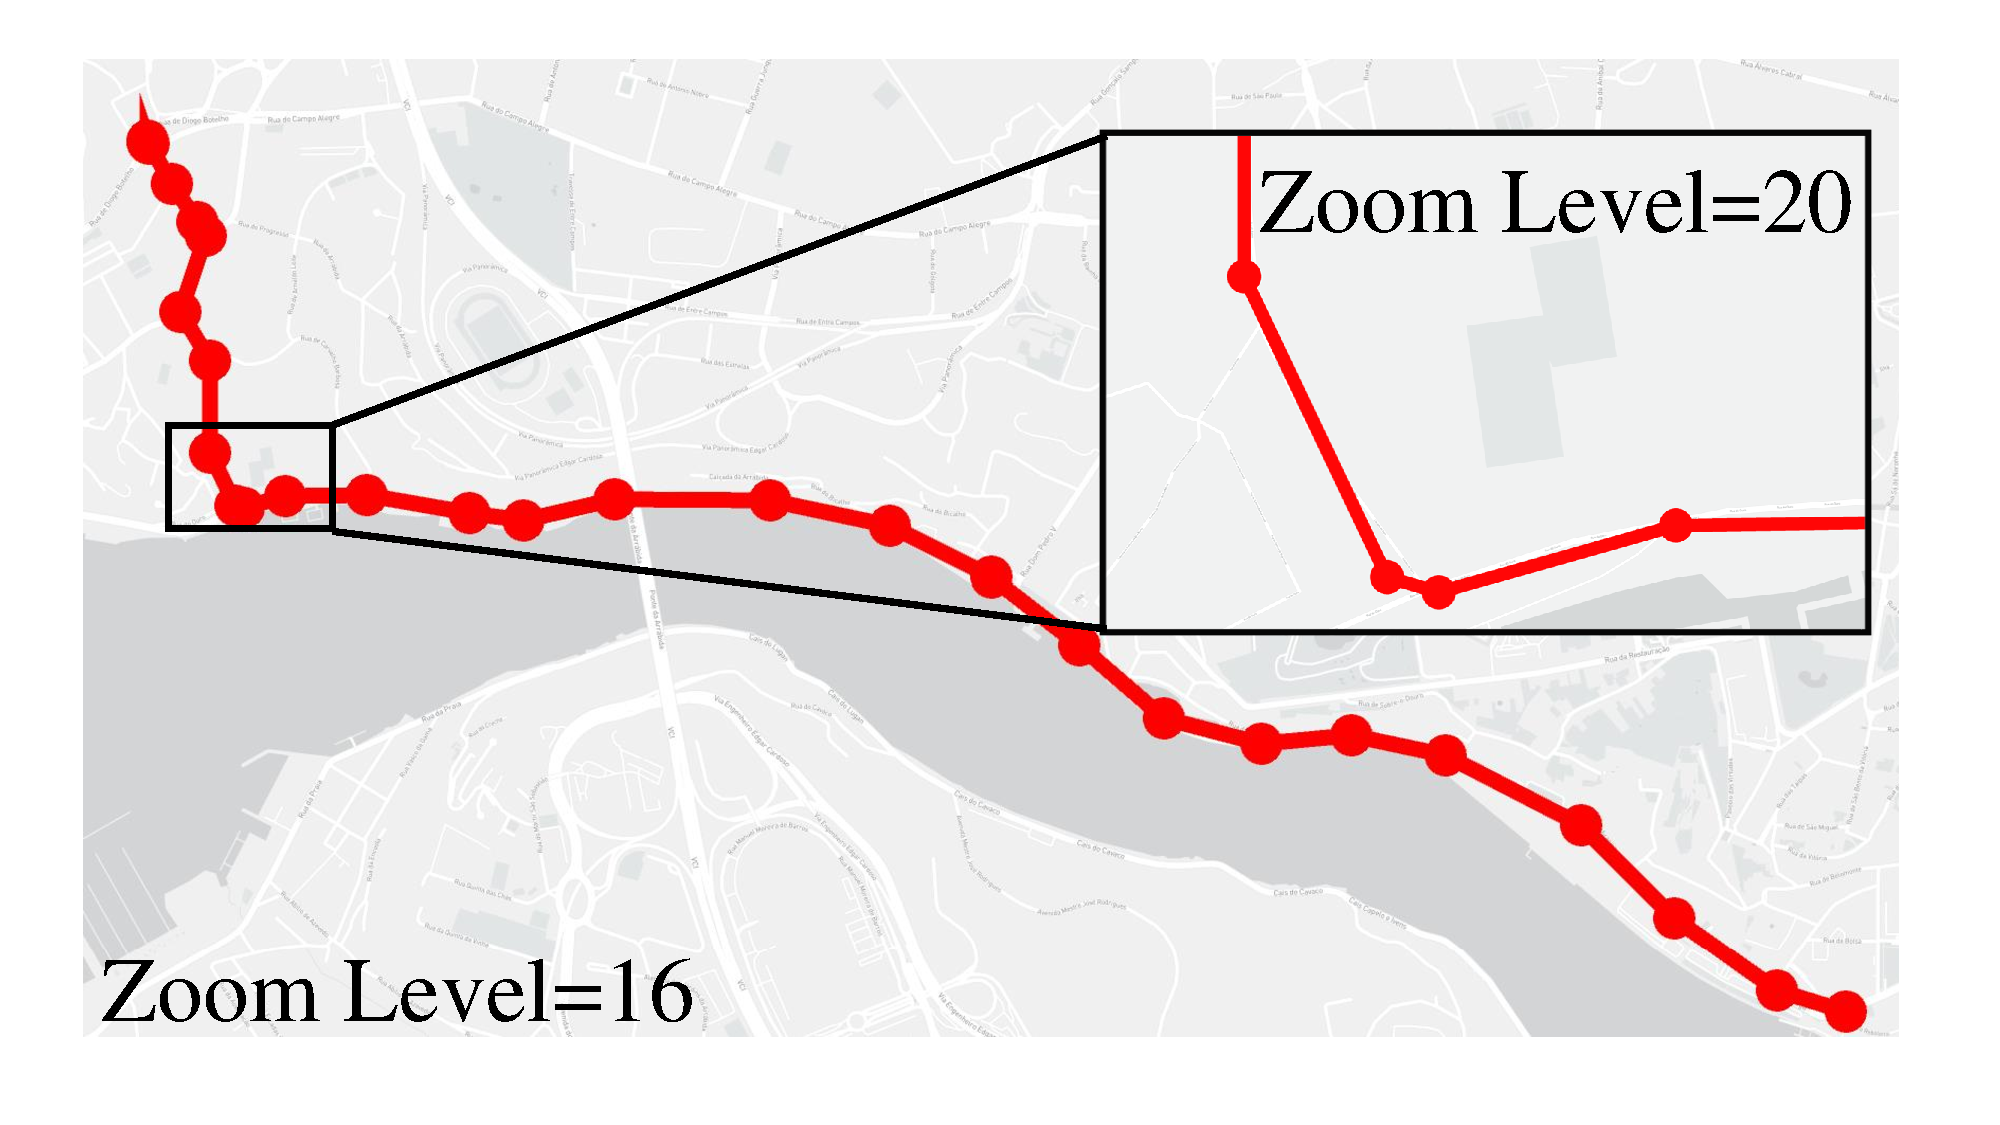
\includegraphics[width=0.48\columnwidth]{pictures/problemsolveing/TrajZoomIn}		
		\\
		(A) Line-based visualization
		&
        (B) Zoom levels
	\end{tabular}
	\vspace{-2mm}
	\caption{Illustration of line-based trajectory visualization.} \label{fig:line}
	\vspace{-2mm}
\end{figure}


\subsection{Problem Definition}\label{sec:def}


We motivate our definition of the \textit{fidelity loss function} by introducing how line-based trajectory visualization works. As introduced earlier, a trajectory contains a sequence of 2-dimensional locations. Given an empty canvas (i.e., the screen of a displaying device) with pixels indexed by horizontal and vertical coordinates (i.e., $x$ and $y$), line-based trajectory visualization connects consecutive locations in each trajectory with polylines and marks the pixels passed by these polylines (with a color different from the background). As shown in Figure~\ref{fig:line}(A), the result of line-based trajectory visualization can be regarded as a 2-dimensional array of boolean variables with 1 indicting a pixel has been marked. Alternatively, we can treat a visualization result $\mathcal{V}$ as a set that contains all marked pixels. This observation leads to the following definition of the fidelity loss function
\begin{equation}\label{eqref:loss}
loss(\mathcal{V}, \mathcal{V}')=\frac{|\mathcal{V}-\mathcal{V}'|}{|\mathcal{V}|},
\end{equation}
in which $|.|$ measures the cardinality of a set, and set $\mathcal{V}^\star=\mathcal{V}-\mathcal{V}'$ contains all distinct elements between $\mathcal{V}$ and $\mathcal{V}'$. We use $loss(\mathcal{V}, \mathcal{V}')$ to measure the fidelity loss of a visualization result $\mathcal{V}'$ compared to the ground-truth visualization $\mathcal{V}$. This definition matches human visual perception as it is essentially the ratio of different pixels in two visualization results. Thus, the approximate visualization $\mathcal{V}'$ will look similar to $\mathcal{V}$ if $loss(\mathcal{V}, \mathcal{V}')$ is small.


Given the fidelity loss function, we are ready to define the fidelity-optimal sampling problem. Denote the set of all trajectories in a dataset as $\mathcal{T}$ and a subset of $\mathcal{T}$ (which contains some sampled trajectories) as $\mathcal{R}$. With a slight abuse of the notation, we use $V(\mathcal{S})$ to denote the visualization results derived from a set $\mathcal{S}$ of trajectories.

\begin{problem}[Fidelity-optimal sampling problem]\label{prob:def}
	Given a sampling rate $\alpha$, find a set $\mathcal{R}$ that satisfies
	\begin{equation}\label{eq:opp}
	\min_{\mathcal{R} \subseteq \mathcal{T}, |\mathcal{R} | = \alpha \mathcal{T} } loss(V(\mathcal{T}), V(\mathcal{R})).
	\end{equation}
\end{problem}
If there is a solution for the above fidelity-optimal sampling problem, to provide a guaranteed fidelity $loss(V(\mathcal{T}), V(\mathcal{R}))\le \tau$, we can simply use a binary search to find the smallest $\alpha$ under which the visual fidelity requirement holds.

One subtlety is that trajectory visualization needs to work at different \textit{zoom levels} upon user request. For example, Google map~\cite{googlemap} provides a zoom levels from 0 to 20, with level 0 providing the largest visualization range (i.e., the whole world) but the lowest resolution, and level 20 providing the smallest visualization range (e.g., individual building, if available) but the highest resolution. We also provided an illustration of zoom level in Figure~\ref{fig:line}(B). Ideally, we want a sample to be \textit{zoom-level-independent}, providing a consistent fidelity guarantee at different zoom levels. This turns out to be straightforward as trajectory visualization merges several pixels in a high-level result (by pixel-wise $OR$) to obtain a pixel in a lower-level visualization result. The following theorem shows that it suffices to satisfy the fidelity guarantee at the highest zoom level.
\begin{theorem}~\label{the:level}
	Use~$loss(V(\mathcal{T}), V(\mathcal{R}), l)$ to denote the fidelity loss induced by a sample set $\mathcal{R}$ at zoom level $l$, we have~ $loss(V(\mathcal{T}), V(\mathcal{R}), l) \\ \le loss(V(\mathcal{T}), V(\mathcal{R}), l')$ if $l\le l'$~\footnote{We omitted the proofs of all theorems and lemmas due to space limit, and refer the interested readers to our technical report~\cite{techreport}.}, with larger $l$ indicating higher resolution.
\end{theorem}
We are aware that lower zoom levels need more coarse-grained visualization and thus the sampling rate at the highest level may be larger than necessary. We left more sophisticated designs, such as re-sampling a sample set or generating multiple sample sets for future work, and consider only sampling for the highest zoom level. As our fidelity loss function considers the entire visible region (i.e., it is a \textit{global fidelity measure}), the visual difference between our sample and the ground-truth visualization may be large for some specific regions, especially when the marked points are sparse in these regions. \textit{Local visual fidelity} can be important for some tasks(e.g., outlier discovery~\cite{feng2010matching,mayorga2013splatterplots}) and we leave it for future work. We want to note that a fidelity-guaranteed sample $\mathcal{R}$ is also \textit{query independent} from the definition of the fidelity loss function, which means $\mathcal{R}$ only needs to be constructed once to answer all queries.






\subsection{Hardness Analysis}\label{sec:hard}
We use $t_i \in \mathcal{T}$ to denote a trajectory in the dataset. According to the working mechanism of line-based trajectory visualization, $t_i$ corresponds to a set of marked pixels on the canvas in the ground-truth visualization and we also use $t_i$ to denote this set of pixels. Thus, we have $V(\mathcal{T}) = \cup_{t_i \in \mathcal{T}} t_i$ and $V(\mathcal{R}) = \cup_{t_i \in \mathcal{R}} t_i$. We can transform Problem~\ref{prob:def} as follows

\begin{align}\label{eqn:obj2} \nonumber
\min_{\oR \subseteq \D, |\oR| = \alpha |\D|}  \frac{|\V(\D) - \V(\oR)|}{|\V(\D)|}  & \Leftrightarrow \min_{\oR \subseteq \D, |\oR| = \alpha |\D|}   - |\V(\oR)| \\ \nonumber
 \Leftrightarrow \max_{\oR \subseteq \D, |\oR| = \alpha |\D|}  |\V(\oR)| &  \Leftrightarrow \max_{\oR \subseteq \D, |\oR| = \alpha |\D|} | \cup_{t_i \in \oR} t_i |
\end{align}

The above transformations use the fact that $V(\mathcal{R}) \subset V(\mathcal{T})$ as $\mathcal{R} \subset \mathcal{T}$, and the ground-truth set $V(\mathcal{T})$ is constant. The last line shows that fidelity-optimal sampling is equivalent to the well-known set cover maximization problem.
Specifically, given an integer $k = \alpha |\D|$, and a collection trajectory pixel set $\D = \{t_1, t_2, \cdots, t_n \}$, set cover maximization finds a subset $\oR \subset \D$ such that $|\oR| \leq k$ and $|\cup_{t_i \in \oR} t_i|$ is maximized. The set cover maximization problem is well-known to be NP-hard~\cite{setcover}.


%It is equivalent to select sized-$k$ trajectory set $\oR$ from $\D$ which $\cup_{\oR_i \in \oR} \oR_i$ is maximized.
%It is a NP-hard problem as we proved in Lemma~\ref{lem:np}.

%\begin{lemma}[NP hard]~\label{lem:np}
%Given a trajectory dataset $\D$ and an integer $k$,
%The sampling-based trajectory visualization problem (see Problem~\ref{prob:def}) is NP-hard.
%\end{lemma}

%We omit the proof of Lemma~\ref{lem:np} as it is a typical set cover maximization problem\footnote{\url{https://en.wikipedia.org/wiki/Maximum_coverage_problem}}, which is a well-known NP-hard problem in literature.

%------------comments by Bo-------------------
%As we analyzed in Section~\ref{sec:intro}, the large-scale (e.g., hundreds of millions GPS points) line-based trajectory visualization problem is very challenging due to the large data size and limited rendering capability of graphics devices.
%To make matters worse, the visualization result of large-scale trajectory dataset suffers visual clutter seriously.
%In this work, we focus on how to visualize large-scale trajectory dataset efficiently and effectively.
%In particular, our objective is to devise a visual fidelity guaranteed sampling method for large trajectory data visualization.
%The major challenges to achieve this goal are:
%(i) how to define visual fidelity theoretically? (ii) how to guarantee the visual fidelity of the sampling-based visualization result?


\section{Our Solution: $\vats$}\label{sec:sol}
In this part, we address the second technical challenge: \emph{how to devise an efficient sampling algorithm that provides guaranteed visual quality?}
Specifically, we first propose a visual quality-guaranteed sampling algorithm $\vats$ in Section~\ref{sec:greedy}. Next, we devise optimizations to improve the efficiency of $\vats$ in Section~\ref{sec:opt}.

\subsection{Visual quality-Guaranteed Sampling}\label{sec:greedy}
%Due to the hardness of Problem~\ref{prob:def}, the straight-forward solution is uniform random sampling $\rand$.
%This solution randomly selects $k$ trajectories from the dataset $\D$ and stores them in the result set $\oR$. The selected trajectories in $\oR$ are rendered as the visualization result.
%Obviously, uniform random sampling $\rand$ does not provide any guarantee on the visual quality of the sampled set.

Our visual quality-guaranteed sampling method $\vats$ is presented in Algorithm~\ref{alg:greedy}, which employs a greedy paradigm.
In particular, it finds the trajectory $tmp$ in $\D$ that maximizes $| tmp \cup \oR|$ at each iteration, as shown in Line~\ref{line:max} of Algorithm~\ref{alg:greedy}.
It terminates after $k=\alpha |\D|$ iterations and returns $\oR$ as the result set for rendering.

%\vspace{-2mm}
\begin{algorithm}
    \caption{$\vats(\D,k=\alpha |\D|)$} \label{alg:greedy}
    \begin{algorithmic}[1]
    \State Initialize result set $\oR \leftarrow \emptyset$
    \While{$|\oR| < k$}
        \State $tmp \leftarrow argmax_{t_i \in \D} |t_i \cup \oR|$ \label{line:max}
        \State $\oR \leftarrow \oR \cup \{ tmp \}$
    \EndWhile
    \State Return $\oR$
    \end{algorithmic}
\end{algorithm}


Interestingly, Algorithm~\ref{alg:greedy} provides provable visual quality guarantee for the returned result $\oR$, as stated in Theorem~\ref{the:ratio}.
%~\footnote{We omitted all the proofs of the theorems and lemmata in this work due to space reasons, and refer the interested readers to our technical report\cite{techreport}.}

\begin{theorem}~\label{the:ratio}
Define the visual quality of a sample set $\mathcal{S}$ as $f(\mathcal{S})=1-loss(\V(\D),\V(\mathcal{S}))$. Let the sized-k result produced by Algorithm~\ref{alg:greedy} be $\mathcal{R}$ and the sized-k solution of Equation~\eqref{eq:opp} be $\mathcal{R}^{\star}$, we have $f(\mathcal{R})\ge 0.632*f(\mathcal{R}^{\star})$.
\end{theorem}

Theorem~\ref{the:ratio} follows directly from the submodularity of the visual quality function $f(\mathcal{S})$ as it is well known that the greedy solution provides a $0.632$ approximation of the optimal solution for a submodular function. We show that submodularity of $f(\mathcal{S})$ as follows.      

\begin{lemma}[Submodularity]\label{lem:submodular}
	Define the contribution of a trajectory $t$ to the result set $\oR$ as $\Delta(\oR, t) = |V(\oR \cup t)| - |V(\oR)|$.
	Given a trajectory $t$ and two result sets $\oR,\oR^{'}$, if $\oR \subset \oR^{'}$, then $ \Delta(\oR, t) \geq \Delta(\oR^{'}, t)$.
\end{lemma}


%\REPORT{
\begin{proof}
	The contribution value of trajectory $t$ w.r.t. a given result set $\oR$ (i.e., $\Delta(\oR, t) = |V(\oR \cup t)| - |V(\oR)|$) is the newly covered pixels, which can be expressed as $|V(t)| - |V(\oR \cap t)|$.
	We have $t \cap \oR \subseteq  t \cap \oR^{'}$ as $\oR^{'}$ is a superset of $\oR$, which implies $|V(t)| - |V(t \cap \oR)| \geq |V(t)| - |V(t \cap \oR^{'})|$.
	Thus, it holds that $\Delta(\oR, t) = |V(\oR \cup t)| - |V(\oR)| \geq |V(\oR^{'} \cup t)| - |V(\oR^{'})|= \Delta(\oR^{'}, t)$.
\end{proof}
%}


%\begin{proof}
%The optimal solution of Problem~\ref{prob:def} covers $f(\mathcal{R}^{\star})$ pixels in $k$ iterations.
%Let $a_i$ be the number of newly covered pixels at the $i$-th iteration, $b_i$ is the total number of covered pixels up to the $i$-th iteration (i.e., $b_i = \sum_{j=1}^{i}a_i$),
%and $c_i$ be the uncovered pixels after $i$-th iteration (i.e., $c_i = f(\mathcal{R}^{\star})-b_i$).
%According to greedy paradigm, we can conclude the number of newly covered pixels at the $(i+1)$-th iteration is always greater than or equal to $\frac{1}{k}$ of the number of uncovered pixels after the $i$-th iteration, i.e., $a_{i+1} \geq \frac{c_i}{k}$.
%We prove Theorem~\ref{the:ratio} by proving $c_{i+1} \leq (1-1/k)^{i+1} \cdot f(\mathcal{R}^{\star})$.
%It holds $c_1 \leq (1-1/k) \cdot f(\mathcal{R}^{\star})$ as follows.
%\begin{align} \nonumber
%& a_1 \geq c_0 \cdot 1/k = 1/k \cdot f(\mathcal{R}^{\star}) \text{~~~as we concluded~~~} a_{i+1} \geq \frac{c_i}{k}\\ \nonumber
% \Leftrightarrow  & b_1 \geq 1/k \cdot f(\mathcal{R}^{\star})  \Leftrightarrow  -b_1 \leq - 1/k \cdot f(\mathcal{R}^{\star})  \text{~~~as~~~} a_1 = b_1\\ \nonumber
% \Leftrightarrow & f(\mathcal{R}^{\star}) - b_ 1 \leq f(\mathcal{R}^{\star}) - 1/k \cdot f(\mathcal{R}^{\star})  \Leftrightarrow  c_1 \leq (1-1/k) \cdot f(\mathcal{R}^{\star})
%\end{align}
%For inductive hypothesis assume $c_{i} \leq (1-1/k)^i \cdot f(\mathcal{R}^{\star})$. Thus,
%\begin{align} \nonumber
%& c_{i+1} = c_i - a_{i+1} \leq c_i - c_i/k = (1-1/k) \cdot c_i =  (1-1/k)^{i+1} \cdot f(\mathcal{R}^{\star})
%\end{align}
%
%Hence, it holds $c_k \leq (1-1/k)^{k} \cdot f(\mathcal{R}^{\star})$.
%It is equivalent to $b_k = f(\mathcal{R}) \geq (1 - (1-1/k)^{k}) \cdot f(\mathcal{R}^{\star}) \geq (1-1/e) \cdot f(\mathcal{R}^{\star}) \approx 0.632 \cdot f(\mathcal{R}^{\star})$.
%\end{proof}

Although Algorithm~\ref{alg:greedy} provides quality guarantee for the result set $\oR$, it has a high time complexity, which we show in the following analysis.  

 


%With the above theoretical analysis, Algorithm~\ref{alg:greedy} offers a visual quality-guaranteed sampling algorithm for the large-scale trajectory data visualization problem.
%However, as the time complexity analyzed in Lemma~\ref{lem:cost}, it is not scalable to large-scale trajectory datasets (e.g., millions of trajectories).


\begin{lemma}[Time Complexity]~\label{lem:cost}
	Given trajectory dataset $\D$ and an integer $k = \alpha |\D|$, the time complexity of Algorithm~\ref{alg:greedy} is $O(\alpha \cdot m \cdot |\D|^2)$, where $m$ is the maximum length of all trajectories in dataset $\D$.
\end{lemma}


\begin{proof}
	In each iteration,
	Algorithm~\ref{alg:greedy} computes the uncovered pixels of each trajectory in dataset $\D$ with $O(m)$ cost.
	As the dataset $\D$ has $O(|\D|)$ trajectories and Algorithm~\ref{alg:greedy} runs for $k = \alpha |\D|$ iterations, the total cost is $O(k \cdot m \cdot |\D|)=O(\alpha \cdot m \cdot |\D|^2)$.
\end{proof}


The high complexity of Algorithm~\ref{alg:greedy} hurts its scalability for large-scale trajectory datasets. For example, the \pt{} dataset contains 2.39 millions taxi trajectories, and the longest trajectory has 3,490 GPS points.
It takes 413.6 seconds for Algorithm~\ref{alg:greedy} to obtain a result set $\oR$ with sampling rate $0.1\%$.    Obviously, the running time is too long for interactive trajectory exploration.

\subsection{Heap-based Lazy Computation}\label{sec:opt}




\begin{figure}
	\centering
	\small
	\begin{tabular}{cc}
		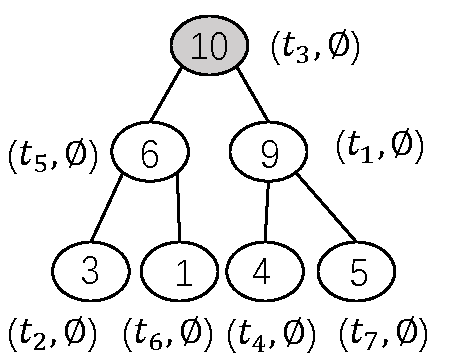
\includegraphics[width=0.35\columnwidth]{pictures/1st}
		&
		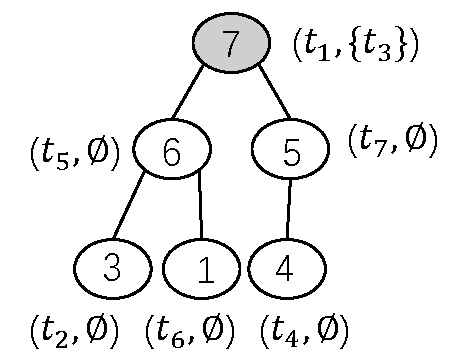
\includegraphics[width=0.35\columnwidth]{pictures/2nd}
		\\
		(A) 1st iteration
		&
		(B) 2nd iteration
	\end{tabular}
	\caption{Lazy computing manner.} \label{fig:heap} %via the submodularity in Lemma~\ref{lem:submodular}
\end{figure}







Algorithm~\ref{alg:greedy} essentially adds the trajectory that maximizes $\Delta(\oR, t) = |V(\oR \cup t)| - |V(\oR)|$ to $\oR$ in each iteration. Lemma~\ref{lem:submodular} shows that the contribution of a trajectory (i.e., $\Delta(\oR, t)$) cannot increase when Algorithm~\ref{alg:greedy} runs for more iterations because $ \Delta(\oR^{'}, t) \le \Delta(\oR, t) $ for  $\oR \subset \oR^{'}$. Based on this property, we can use  $\Delta(\oR, t)$ calculated in the previous iterations to prune a trajectory $t$ from computation. If we have $\Delta(\oR, t)\le \Delta(\oR^{'}, t')$, in which $\oR$ and $\oR^{'}$ are a previous and the current sample set, respectively, we know that $t$ can not be added to the sample set in the current iteration.         

 

To implement this idea, we maintain a max-heap for the number of uncovered pixels of each trajectory and update the max-heap in a lazy fashion. 
That is, the contribution of a trajectory is computed only when necessary.
Figure~\ref{fig:heap}(a) shows a tiny max-heap example for the numbers of uncovered pixels of trajectories from $t_1$ to $t_7$ with result set $\oR=\emptyset$.
At the first iteration, the root node of the max-heap, $t_3$ in Figure~\ref{fig:heap}(A), is selected.
At the second iteration, the number of uncovered pixels of the root node $t_1$ is updated to 7 w.r.t. result set $\oR = \{t_3 \}$ (see the gray node in Figure~\ref{fig:heap}(B)).
Then $t_1$ is selected at the second iteration without computing the number of uncovered pixels for other trajectories, i.e., all white nodes in Figure~\ref{fig:heap}(B).
The reason is that the contributions of these trajectories are all less than 7 according to the submodularity in Lemma~\ref{lem:submodular}.

%In summary, the number of uncovered pixels in each trajectory will only be computed with the latest result set $\oR$ when it is necessary in the lazy computing manner,
%e.g., only $t_1$ will be updated at the 2nd iteration in Figure~\ref{fig:heap}.
%It reduces many unnecessary computations through the lazy updating manner, e.g., all white nodes did not update at the 2nd iteration in the above example.

%We then analyze the time complexity of Algorithm~\ref{alg:greedy} with lazy computing manner in Theorem~\ref{lem:lazy}.
%
%\begin{lemma}[Optimized Time Complexity]~\label{lem:lazy}
%Given trajectory dataset $\D$ and an integer $k= \alpha |\D|$, the time complexity of Algorithm~\ref{alg:greedy} with lazy computing manner is $O(\alpha \cdot m \cdot x |\D| \log |\D|)$, where $x$ is the number of contribution computations among all $k$ iterations and $x \ll |\D|$.
%\end{lemma}
%
%\begin{proof}
%It first takes $O(|\D|)$ time to construct the max-heap~\cite{cormen2009introduction}.
%It incurs $O( m \cdot x \log |\D|)$ cost to select the trajectory with maximum uncovered pixels at each iteration ($k$ iterations in total).
%Hence, the overall cost is $O(|\D| + k \cdot m \cdot t \log |\D|)$.
%\end{proof}


The efficiency of Algorithm~\ref{alg:greedy} is significantly improved with heap-based lazy computation.
To exemplify, Algorithm~\ref{alg:greedy} takes 413.6 seconds to return the results with sampling rate $0.1\%$ on the \pt{} taxi trajectory dataset. In contrast, our performance-optimized $\vats$ needs only 1.2 seconds.


\section{Advanced Approach: $\avats$}\label{sec:aa}

In the previous section, we presented the $\vats$ algorithm, which produces quality-guaranteed samples and runs efficiently. 
In this section, we focus on the third technical challenge: \emph{how to tackle the visual clutter problem in large trajectory visualization}?
In particular, we devise an advanced approach $\avats$ by considering
(i) trajectory data distribution, and (ii) human perception capability.
We elaborate (i) and (ii) by the examples in Figure~\ref{fig:delta}.


\stitle{Trajectory data distribution} Considering the \pt{} trajectory dataset, Figure~\ref{fig:delta}(A) is the visualization result of $\vats$ with sampling ratio $0.5\%$. It is obvious that the trajectories follow a non-uniform distribution, and there are some dense regions and sparse regions as illustrated by the rectangles in Figure~\ref{fig:delta}(A).

      
%Obviously, the real-world trajectory dataset is non-uniform distributed.
%For example, the trajectories in dense region are much more than those in the sparse region, as illustrated by the rectangles in Figure~\ref{fig:delta}(A).

\stitle{Human perception capability} Comparing Figures~\ref{fig:delta}(A) and (B), it is easier to tell their differences in the sparse regions than in the dense regions. This is because human beings have limited  perception capability, and hence two visualizations look indistinguishable if both of them contain a large number of points in the same area. This is exactly the case for the two dense regions in Figures~\ref{fig:delta}(A) and (B).       




\begin{figure}%[t]
	\centering
	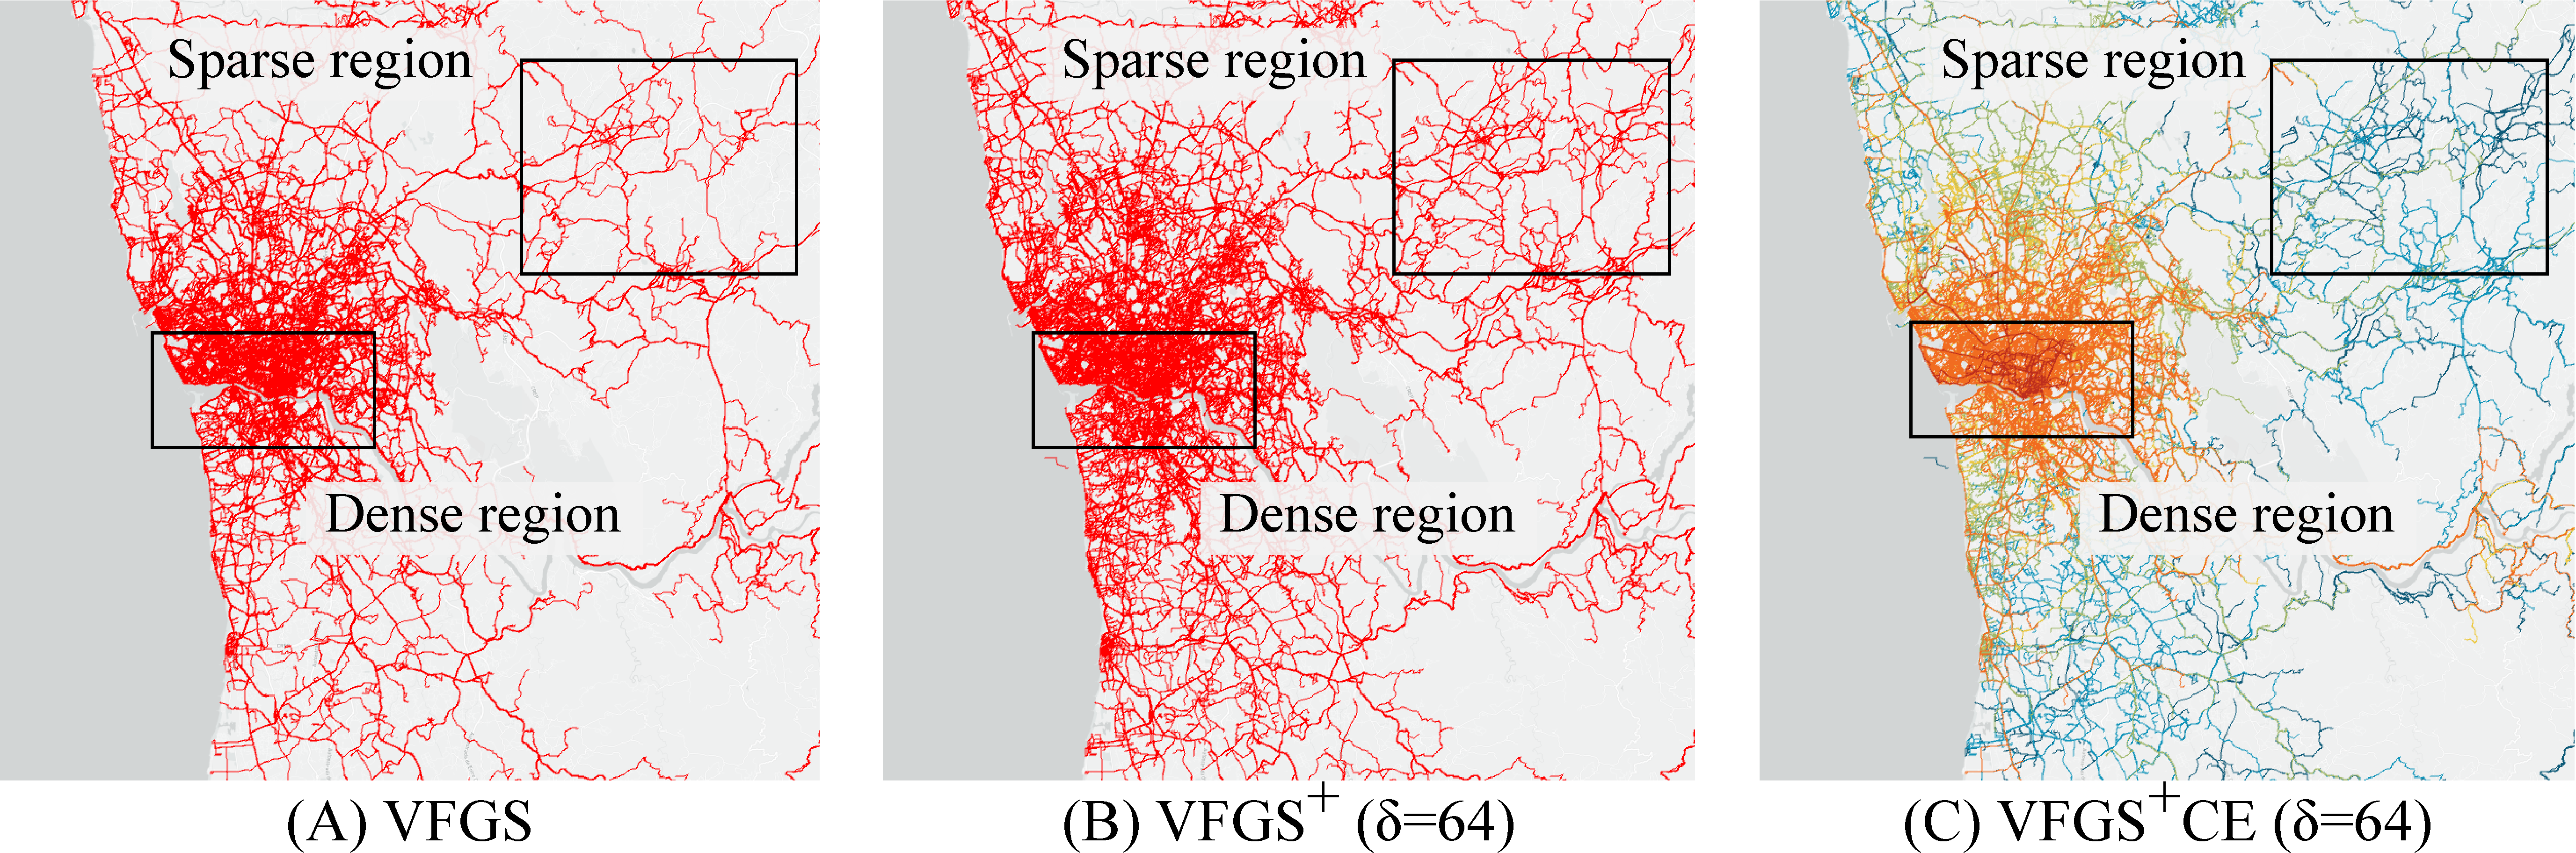
\includegraphics[width=0.48\textwidth]{pictures/problemsolveing/delta_motivation.pdf}
	\caption{The advanced approach $\avats$ on \pt{} ($\alpha = 0.5\%$).} 
	\label{fig:delta}
\end{figure}

%(see Algorithm~\ref{alg:plus})

Based on the two observations above, we can improve  $\vats$ by delivering richer information in the sparse regions and reducing visual clutter in the dense regions. $\avats$ in Algorithm~\ref{alg:plus} achieves both objectives using a perception tolerance parameter $\delta$, which models the perception capability of humans at the highest level of details.
Specifically, if pixel $(x,y)$ in canvas is covered by the result set $\oR$ at the highest level,
the pixels around $(x,y)$, i.e., from $(x-\delta, y-\delta)$ to $(x+\delta, y+\delta)$, does not need to be covered as  they are in the perception tolerance of human beings. We can easily modify $\vats$ in Algorithm~\ref{alg:greedy} to incorporate the perception tolerance parameter $\delta$ as shown in Algorithm~\ref{alg:plus}. $\avats$ measures the contribution of each trajectory $t_i$ w.r.t the augmented set $\oR^{+}$ in Line~\ref{line:deltamax},
where $\oR^{+}$ includes both the selected trajectories and their tolerance pixels (in Line~\ref{line:delta}).      

  
%Taking the above two observations into consideration, we can further improve the returning result of visual quality-guaranteed sampling approach $\vats$ by
%delivering rich information at sparse regions and reducing visual clutter in dense regions.
%In this section, we devise the advanced approach $\avats$ (see Algorithm~\ref{alg:plus}) to achieve the above two objectives.
%In specific, we introduce perception tolerance parameter $\delta$ in $\avats$, which models the perception capability of humans at the highest level of details.
%In other words, suppose the pixel $(x,y)$ in canvas is covered by the result set $\oR$ at the highest level,
%the pixels around $(x,y)$, i.e., from $(x-\delta, y-\delta)$ to $(x+\delta, y+\delta)$, are not necessary to cover because they are in the perception tolerance of human beings.


%It measures the contribution of each trajectory $t_i$ w.r.t the selected trajectory set $\oR$'s augmented set $\oR^{+}$, i.e., the selected trajectories and their tolerance pixels.
%.
%The augmented set $\oR^{+}$ will be updated by the selected trajectory $tmp$ and its tolerance pixels set (in Line~\ref{line:delta}).

%
\begin{algorithm}
    \caption{$\avats(\D,k=\alpha |\D|,\delta)$} \label{alg:plus}
    \begin{algorithmic}[1]
    \State Initialize result set $\oR \leftarrow \emptyset$
    \State Initialize augmented result set $\oR^{+} \leftarrow \emptyset$
    \While{$|\oR| < k$}
        \State $tmp \leftarrow argmax_{t_i \in \D} | t_i  \cup \oR^{+} |$ \label{line:deltamax}
        \State $\oR \leftarrow \oR \cup \{ tmp \}$
        \State $\oR^{+} \leftarrow \oR^{+} \cup \mathsf{augment}(tmp, \delta)$\label{line:delta}
    \EndWhile
    \For{each $t$ in $\D$} \Comment{Representative encoding} \label{line:s}
        \State $tr \leftarrow argmin_{t_i \in \oR}{|t-\mathsf{augment}(t_i, \delta)|}$
        \State $tr.\mathsf{cnt}++$ \label{line:e}
    \EndFor
    \State Return $\oR$
    \end{algorithmic}
\end{algorithm}


%Interestingly, the visual clutter large trajectory visualization problem can be further reduced
%by encoding representative trajectories in $\oR$ (the returning result of $\avats$) with colors.
%In particular, $\avats$ selects the trajectory with the largest uncovered pixels by taking the perception tolerance capability of humans into account at each iteration,
%instead of only choosing the trajectory with the largest uncovered pixels in $\vats$ (Algorithm~\ref{alg:greedy}).


$\vats$ in Algorithm~\ref{alg:greedy} selects trajectories with good representativeness and some trajectories will not be included into the result set $\oR$ even though they have more uncovered pixels w.r.t. $\oR$. The reason is that their uncovered pixels are too close to the pixels in the selected trajectories (i.e., within the tolerance area of selected pixels). Take Figure~\ref{fig:zoom}(A) for example, suppose $\delta=1$ and trajectory $a$ was selected at the first iteration, the trajectory to select in the second iteration is $c$ instead of $b$ because almost all pixels in $b$ is in the tolerance area of $a$'s. $\avats$ also provides excellent visual quality at arbitrary zooming resolutions. This is because it considers the perception tolerance parameter $\delta$  at the highest zoom level. For example, the zoom level in Figure~\ref{fig:zoom}(A) is higher than that in Figure~\ref{fig:zoom}(B).
According to our elaboration, $\avats$ selects trajectory $a$ and $c$ for Figure~\ref{fig:zoom}(A).
When the area is zoomed out, as shown in Figure~\ref{fig:zoom}(b), trajectory $a$ and $c$ still captures the main sketch of the underlying dataset (as gray cells shown).
We will further elaborate this phenomenon by the experimental study in Section~\ref{sec:exp}.



The visual clutter problem for large-scale trajectory visualization can be further alleviated by encoding the representativeness of the trajectories in $\oR$ with colors. We define the representativeness of a trajectory $t_i$ in $\oR$ as the number of trajectories in the dataset $\D$ that has $t_i$ as its nearest neighbor in $\oR$. The distance between trajectory $t$ and $t_i$ is defined as the number of pixels in $t$ that can not be covered by the augmented pixels of $t_i$. We compute the representativeness of each trajectory in $\oR$ from Line~\ref{line:s} to Line~\ref{line:e} in Algorithm~\ref{alg:plus}. Figure~\ref{fig:delta}(C) shows the visualization result by encoding trajectories with larger representativeness with warmer colors. There are more details in the sparse regions compared with the $\vats$ result in Figure~\ref{fig:delta}(A), and we can identify the main roads in the dense region with very warm colors.

%Thus, the selected trajectories in the dense region are more representative than those in sparse region.

\begin{figure}[t]
	\centering
	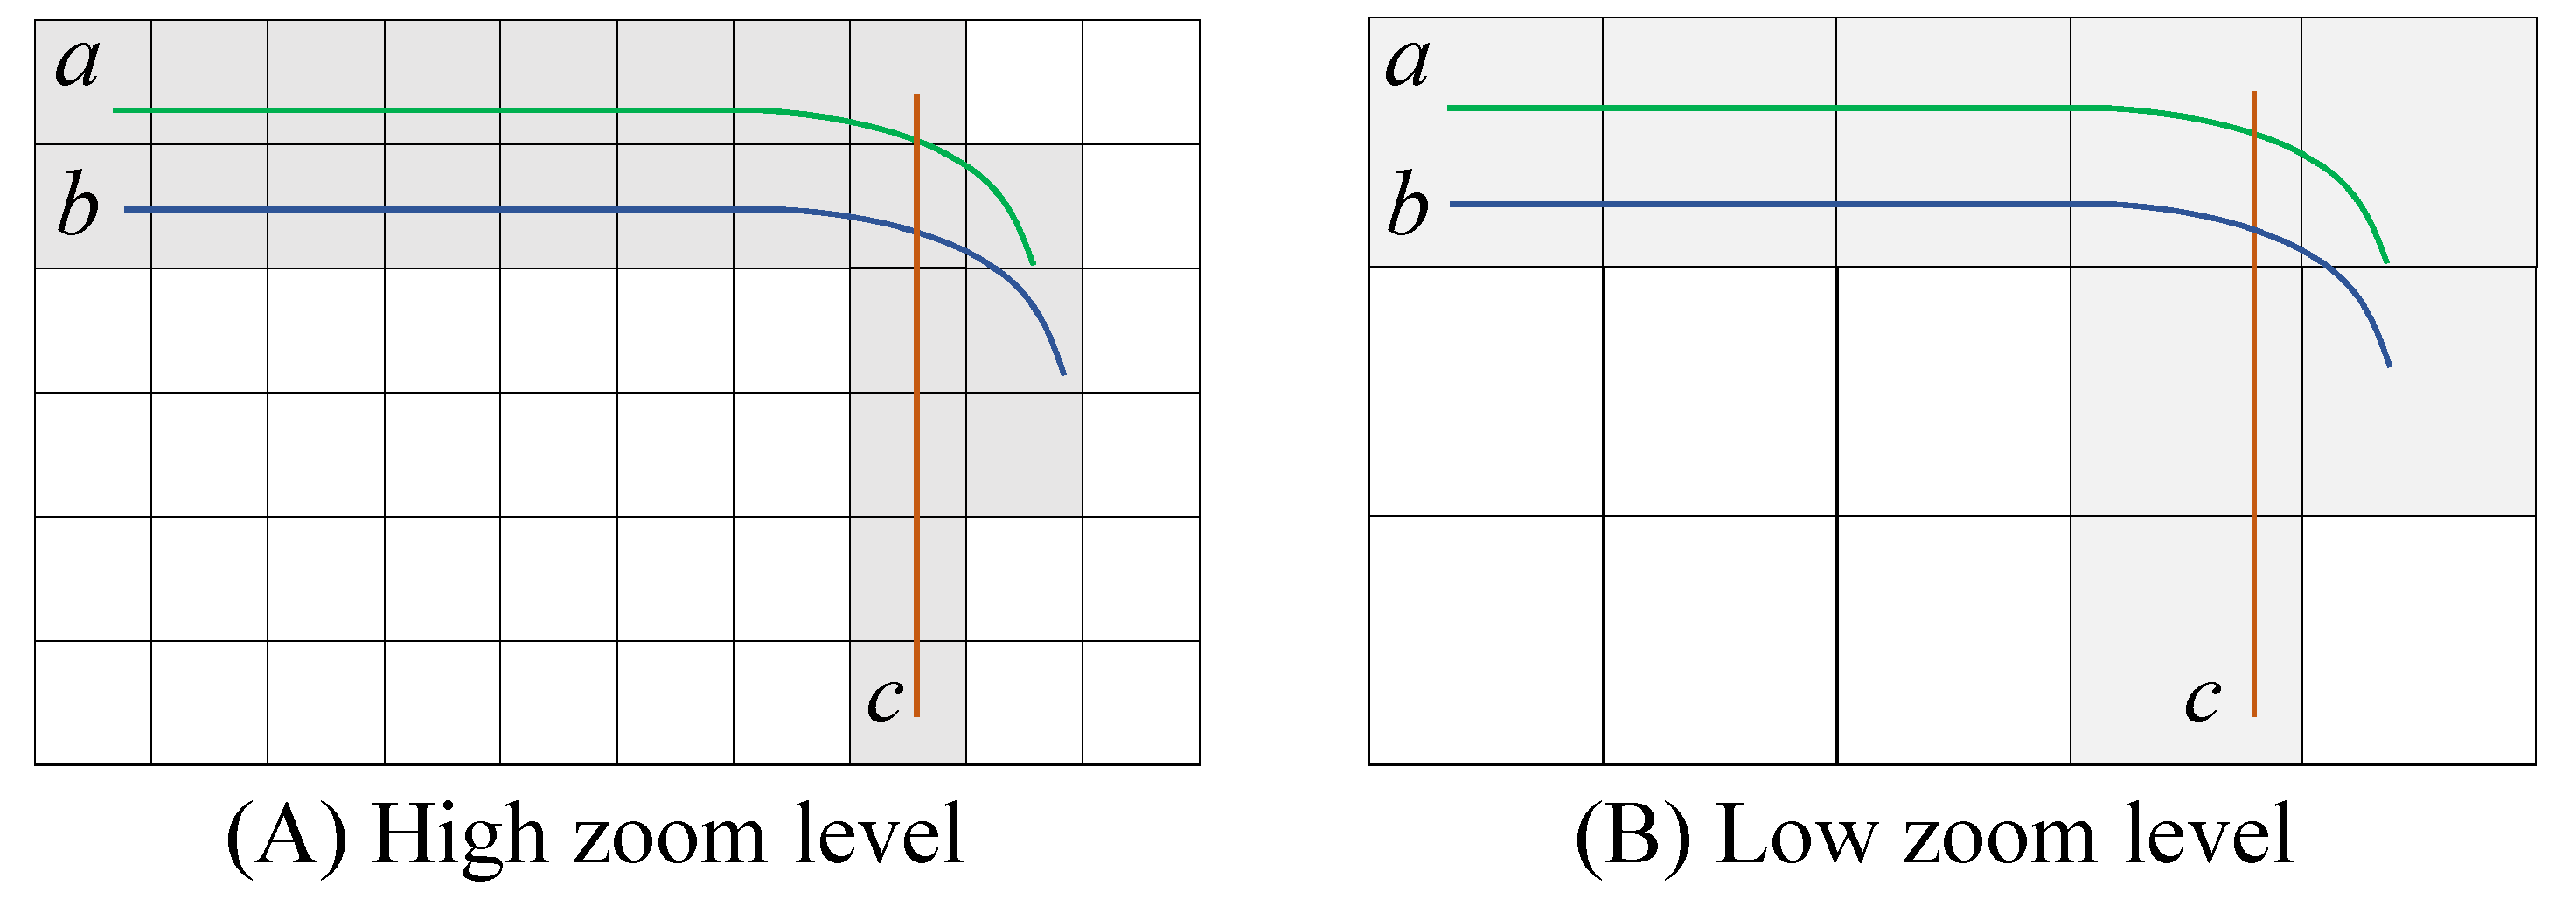
\includegraphics[width=0.45\textwidth]{pictures/problemsolveing/one_to_many.pdf}
	\vspace{-2mm}
	\caption{$\avats$ at different zoom levels.}	\label{fig:zoom} %An illustration of
    \vspace{-2mm}
\end{figure}






%(1) Richer Information Delivering: details aware; so Arbitrary zooming resolutions
%(2) Popularity Embedding: visual clutter



%\subsection{One-to-many strategy}~\label{sec:one_to_many}
%Since we detect the covered pixels in the highest level, two trajectories may be very close to each other but share very few pixels, which will lead to more information loss in the low zoom view as figure~\ref{fig:one_to_many}.
%We next elaborate a ``one-to-many'' strategy to further optimize the visual quality of our proposed technique.
%Recalling we use the highest zoom level to define the pixel size in the canvas.
%Thus, our visual quality guaranteed sampling algorithm is zoom-level oblivious, e.g., it guarantees the visual quality of result set $\oR$ at every zoom level.
%However, users always do not use/need the highest zoom level in visualization applications.
%For example, Google map shows city and streets at zoom level 1 and 15, respectively~\footnote{\url{https://developers.google.com/maps/documentation/}}.
%Motivated by the above observation, we devise ``one-to-many'' strategy by introducing a visual tolerance parameter $\delta$ to optimize the visual quality for users.
%Specifically, ,
%the ``one-to-many'' strategy will ignore all the pixels around $(x,y)$ within $\delta$ offset distance, i.e., all pixels from $(x-\delta, y-\delta)$ to $(x+\delta, y+\delta)$ will be skipped.
%We will demonstrate the effectiveness of the visual tolerance $\delta$ in experimental evaluations.
%
%%https://developers.google.com/maps/documentation/maps-static/dev-guide#Zoomlevels
%\begin{figure}[t]
%	\centering
%	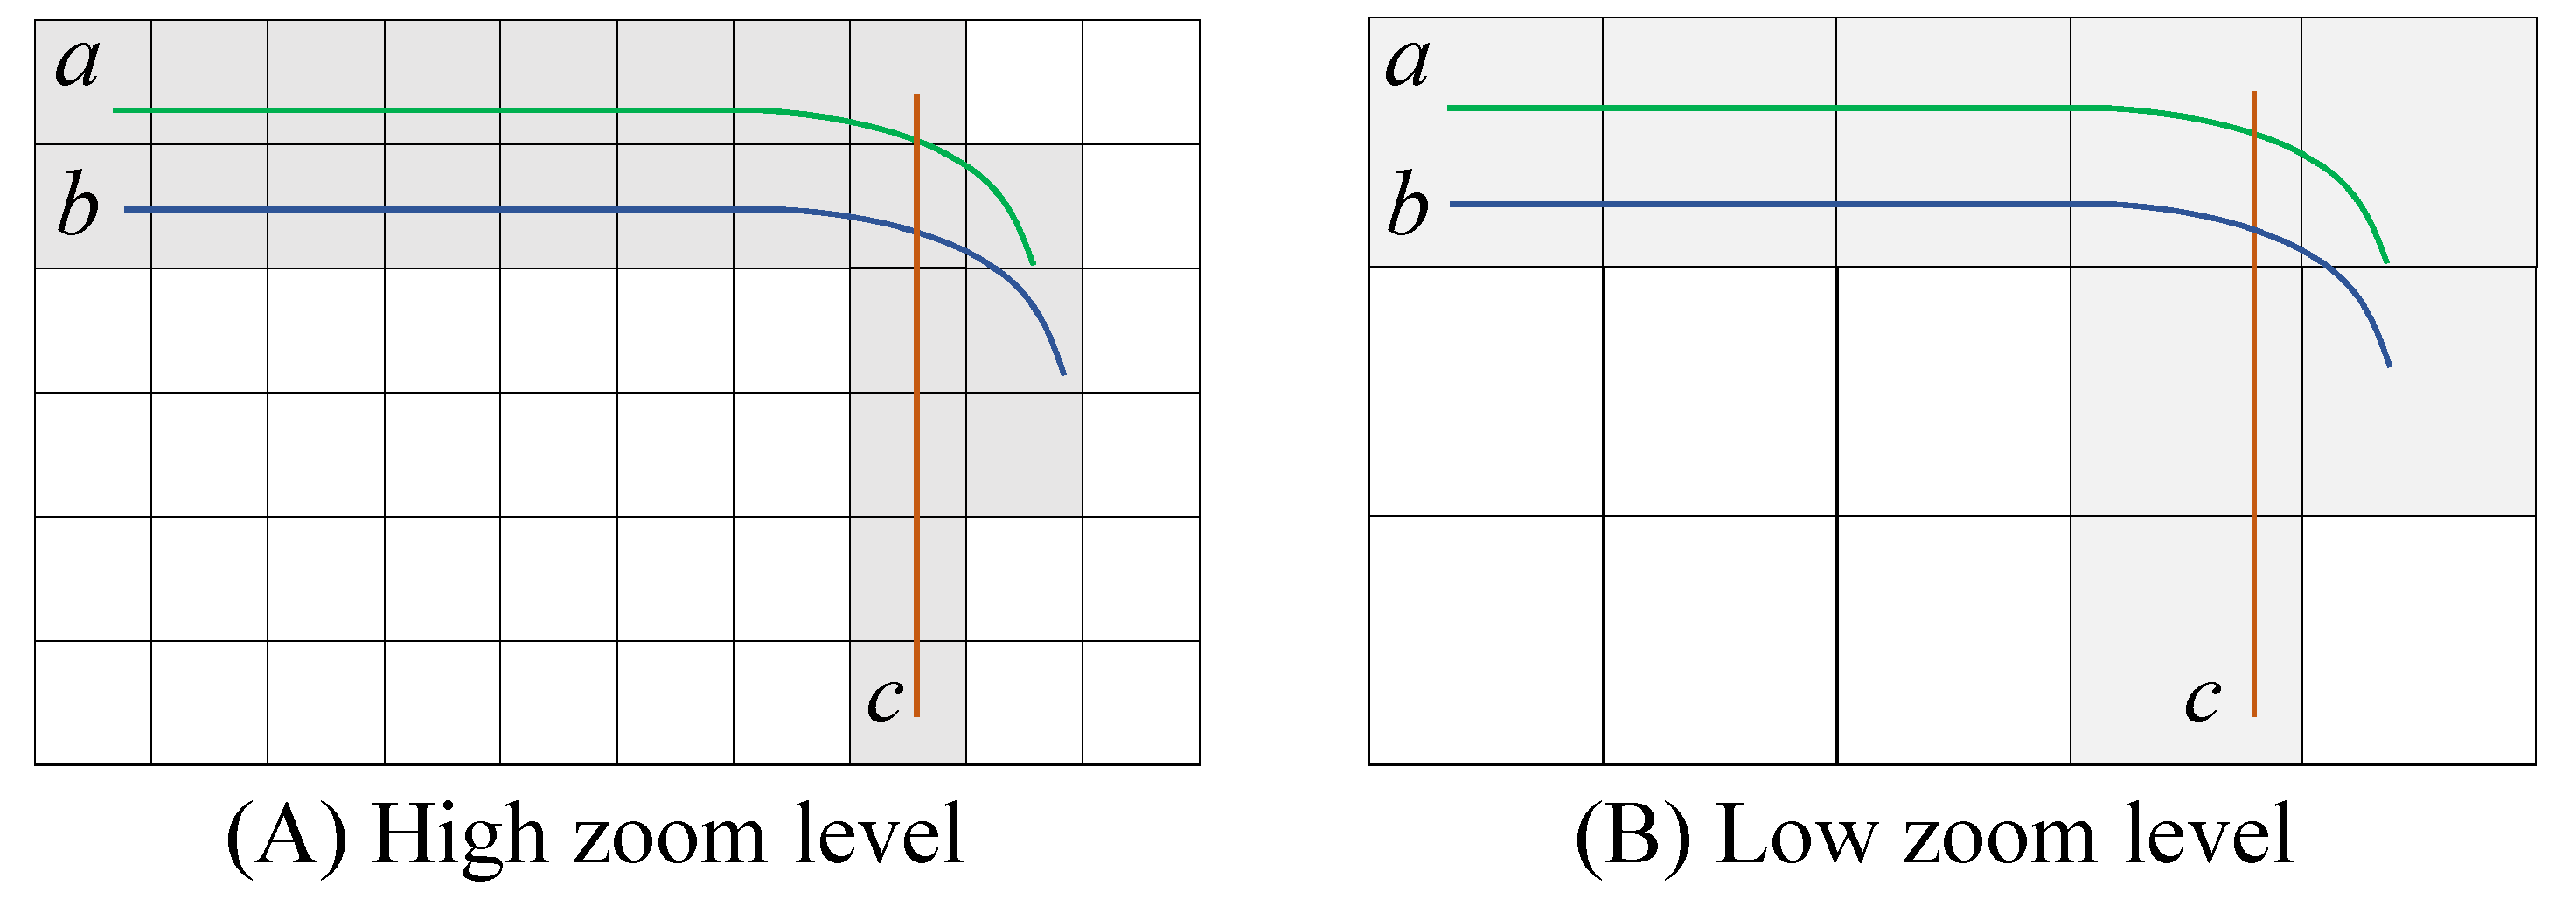
\includegraphics[width=0.4\textwidth]{pictures/problemsolveing/one_to_many.pdf}
%	\vspace{-5mm}
%	\caption{Resolution inconsistency}
%	\vspace{-5mm}
%	\label{fig:one_to_many}
%\end{figure}


%Specifically, $\avats$ incorporates a parameter $\delta$ during trajectory selection process in $\vats$ .
%In particular, we employ the parameter $\delta$ to model the end user's perception ability at the most high level of details.
%Surprisingly, our advance approach $\avats$ not only provides better visualization result when comparing with $\vats$ with the same sampling rate
%(e.g., Figure~\ref{fig:delta}(a) and (b) are the returning result of $\vats$ and $\avats$ respectively),
%but also embeds the popularity of selected trajectories by encoding the rest trajectories in the dataset in them,
%e.g., Figure~\ref{fig:delta}(c) is the visual result of $\avats$ with color encoded popularity.





\section{Experimental Evaluation}\label{sec:exp}
We evaluate our techniques on two real-world trajectory datasets: \pt{}, \sz{} and \cd{}.
\pt{}~\cite{pt} contains a total of 2.39 million taxi trajectories and 75.67 million of GPS points, and the longest trajectory has 3,490 GPS points.
\sz{}~\cite{sz} consists of 3.07 million taxi trajectories with 53.53 million GPS points, and the longest trajectory has 2,268 GPS points. 
\cd{}~\cite{cd} consists of \QM{0.28} million taxi trajectories with \QM{6.69} million GPS points, and the longest trajectory has \QM{4025} GPS points.  All experiments are conducted on a machine with an Intel i7-8700 CPU, 24 GB memory and an NVIDIA GeForce GTX1080 GPU with 8 GB on-chip memory, running on Windows 10. All methods are implemented in Java 1.8, and the Processing 3 library~\cite{p3} is used for rendering. All datasets and source codes required to reproduce our results are available at~\cite{code}.

%\REPORT{
This section is organized as follows.
In Section~\ref{sec:case}, we present several case studies of the visualization results on the \pt{} datasets to demonstrate the merits of our methods.
% In Section~\ref{sec:case}, we evaluate the effectiveness of our proposal by the case studies on \pt{} and \sz{} trajectory dataset, respectively.
%}
In Section~\ref{sec:user}, we conduct a comprehensive user study to test the effectiveness of our visualization results on practical tasks including \textit{region center identification}, \textit{reachable route inspection} and \textit{traffic flow comparison}. In Section~\ref{sec:quality}, we quantitatively evaluate the visual quality and efficiency of our methods on all these three datasets.

% and has been cleaned for further analysis.
\trim \trim



\subsection{Case studies}\label{sec:case}
\subsubsection{Effectiveness of overview visualization}

We conduct case study in \pt{}, shown as the visualization results in Figure~\ref{fig:overview}, to demonstrate the effectiveness our proposals from the following aspects.

\stitle{Consistently good visual quality at overview}
At zoom level 11, Figure~\ref{fig:overview}(A) is the visualization result of the full \pt{} dataset.
With a sampling rate $\alpha \!=\! 1\%$, Figures~\ref{fig:overview}(B) and (C) are the visualizations produced by uniform random sampling ($\rand$), $\baseline$~\cite{borcan2012improving},   
and our visual quality-guaranteed sampling method ($\avats$, \QM{Algorithm~\ref{alg:plus}}), respectively. Comparing with Figure~\ref{fig:overview}(B) and (C), it is obvious that Figure~\ref{fig:overview}(E) is more similar to Figure~\ref{fig:overview}(A). In particular, Figure~\ref{fig:overview}(E) not only preserves the overall visual structure of the entire region but also keeps the details of cities that are far from the center (marked by the dashed cycles in the figure). However, the details of these cities are lost in Figure~\ref{fig:overview}(C) as $\rand{}$ mostly preserve trajectories in the dense region. \QM{On the other sides, the distance based sampling keeps the trajectories in the sparse regions but cannot guarantee visual quality.} 

\stitle{Consistently good visual quality under different sampling rates}
Figures~\ref{fig:overview}(D) and (E) are the visualizations produced by $\avats{}$ with a sampling rate of $0.1\%$ and $1\%$. We can make two observations: (i) the larger the sampling rate, the better the visual quality, i.e., Figures~\ref{fig:overview}(C) and (E) are more similar to Figure~\ref{fig:overview}(A) compared with Figures~\ref{fig:overview}(B) and (D); (ii) the visualization of $\avats$ with a sampling rate of $0.1\%$ (i.e., Figure~\ref{fig:overview}(D)) looks even more appealing than the visualization of $\rand{}$ with a sampling rate of $1\%$ (i.e., Figure~\ref{fig:overview}(C)) as Figure~\ref{fig:overview}(D) better captures the overall visual structure of Figure~\ref{fig:overview}(A).

%Figures~\ref{fig:teaser}(D) and (E) are the visualizations produced by $\rand{}$ with a sampling rate of $0.1\%$ and $1\%$, respectively, while Figures~\ref{fig:teaser}(D) and (E) are the visualizations generated by our $\avats{}$ algorithm at the same sampling rates. We can make two observations: (i) the larger the sampling rate, the better the visual quality, i.e., Figures~\ref{fig:teaser}(C) and (E) are more similar to Figure~\ref{fig:teaser}(A) compared with Figures~\ref{fig:teaser}(B) and (D); (ii) the visualization of $\avats$ with a sampling rate of $0.1\%$ (i.e., Figure~\ref{fig:teaser}(D)) looks even more appealing than the visualization of $\rand{}$ with a sampling rate of $1\%$ (i.e., Figure~\ref{fig:teaser}(C)) as Figure~\ref{fig:teaser}(D) better captures the overall visual structure of Figure~\ref{fig:teaser}(A).

\stitle{Color encoding effectively mitigates visual clutter}
% Then, we present the superiority of the color encoding scheme in $\avats$, which denotes as $\cavats$ in subsequent sections.
At a zoom level of 11 and with a sampling rate of $1\%$, Figures~\ref{fig:overview}(E) and (F) are the visualizations produced our $\avats$ and $\cavats$ (i.e., $\avats$ with color encoding), respectively.
Visual clutter is severe for the full dataset (i.e., Figure~\ref{fig:overview}(A)) and Figures~\ref{fig:overview}(E) since almost all pixels in the center regions are colored, and it is difficult to identify patterns in the these regions. The visualization of $\cavats$ in Figure~\ref{fig:overview}(F) migrate this problem by encoding the trajectories with color, and thus it is easy to identify some prominent trajectories and busy routes. 


\subsubsection{Case Studies on the effectiveness of detail view}\label{sec:detail}


\begin{figure*}[t]
	\centering
	\includegraphics[width=0.95\textwidth]{pictures/case_study_icde/case_study_detail.pdf}
	\vspace{-3mm}
	\caption{Effectiveness studies of $\qtavats$ at detail visualization.}
	\label{fig:detailview}
	\vspace{-2mm}
\end{figure*}

We next present the effectiveness of our proposals with detail views by investigating two regions of interest in \pt{}, the dense region B and the sparse region C(shown as in Figure~\ref{fig:detailview}(8)).

\stitle{Dense region}
Region B is the center of Porto with the zoom level of 15, which has the highest concentration of the trajectories and causes serious visual clutter, as visualized in Figure~\ref{fig:detailview}(B1).
For example, the circular structures of the main route(shown as the dash circular region in Figure~\ref{fig:detailview}(B1)) is unclear.
$\localavats$ alleviates the visual clutter by preserve the $1\%$ trajectories of the total regions but the clutter is still serious. Furthermore, $\avats$ performs better than $\localavats$ by preserving less trajectories and reduce the visual clutter. 


\stitle{Sparse region}
Region C includes the city of Casino Espinho at zoom level 14, which contains less trajectories than the center of Porto as the visualization result of full dataset shown in Figure~\ref{fig:detailview}(C1). 
Given fix sampling rate $\alpha=1\%$, Figure~\ref{fig:detailview}(C2) indicates the visualization of $\localavats$. This visualization result misses a lot if detail information in this region, because the fix sampling rate preserves too few trajectories which is difficult to guarantee the visual quality.
While $\avats$ in Figure~\ref{fig:detailview}(C3) performs much better than $\localavats$ as the sampling rate is automatically adjusted to according to the visual quality. In this visualization, the trajectory sketch of Casino Espinho is almost the same as it in Figure~\ref{fig:detailview}(C1), the visualized result of full dataset.

%\subsection{User Study}\label{sec:user}

In this part, we conduct a comprehensive user study to evaluate the quality of visualizations generated by different methods.

\subsubsection{Settings}
We recruited ** participants with ** females, ** males, aged **-** with a mean of ** for the user study. The user study is conducted on the two larger datasets, i.e., \pt{} and \sz{}, and four methods are investigated, i.e., $\full$, $\rand$, $\mathsf{DTW}$ and $\avats$. We manually select 22 \textit{center points} in the two datasets and define 3 \textit{visualization scales} including:
large-scale region (zoom level less than 13), middle-scale region (zoom level between 13 and 15), small-scale region (zoom level more than 15). For each center point and visualization scale, we generate a \textit{comparable visualization group}, which includes one visualization generated by each of the 4 methods. This results in 66 comparable groups (22 center points $\times$ 3 scales) and 264 visualization results (66 comparable groups $\times$ 4 visualizations).

We are interested in the visual quality and visual clutter of the visualization results, and hence designed three tasks for a comparable group: \textit{T1}) rank the visualizations in the group from the highest visual quality to the lowest visual quality by 1-4;
\textit{T2}) rank the visualizations in the group from the least visual clutter to the most severe visual clutter by 1-4;
\textit{T3}) select the acceptable visualizations (multiple choices allowed) for analysis and choose the reason for those that are not selected, and we provide three reasons including ``severe visual clutter", ``poor visual quality" and ``others".  The user study system is a web-based platform, in which all visualizations are displayed with a resolution of 450*300.

\subsubsection{User study procedure}

When the participants enter the user study system, they are given a brief introduction and a tutorial on how to conduct the tasks to get familiar with the interface and tasks.
For each participant, we randomly select 16 comparable groups and generate 48 tasks.
For each comparable group, the 4 visualizations (\textit{without specifying generated by which method}) in one comparable group are shown on the same web-page and a participant is required to perform task T1, T2 and T3 by inspecting them.

%At last, the participants are interviewed to collect feedback after finishing the study and their answers are saved for result analysis.

\subsubsection{Result analysis}

\begin{figure*}[t]
	\centering
	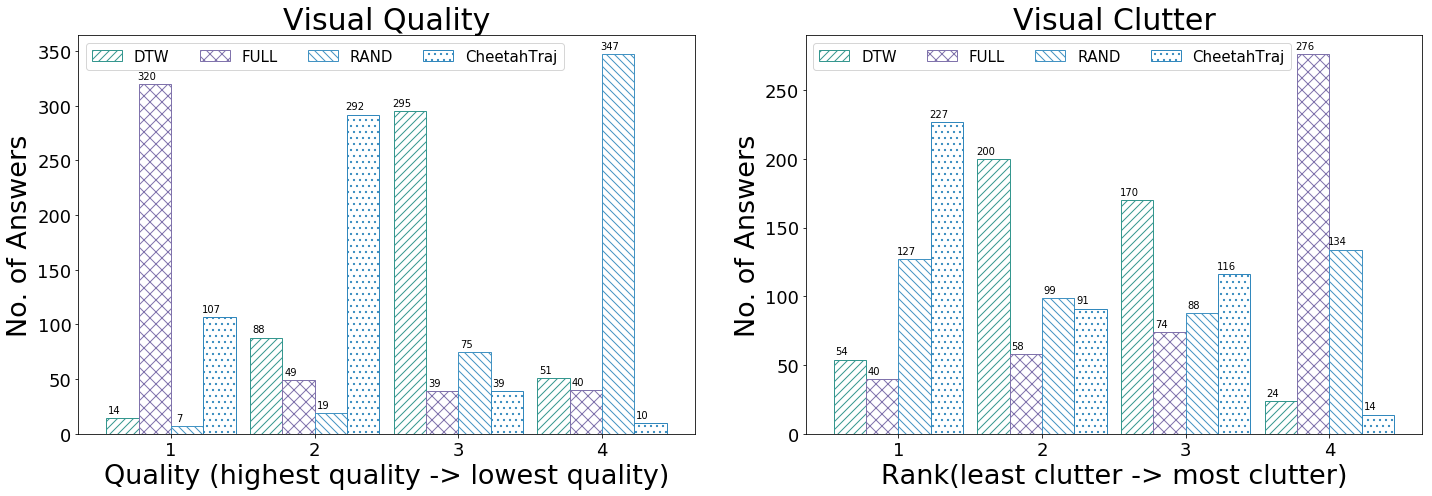
\includegraphics[width=0.6\textwidth]{pictures/user_study/rank.png}
	%\vspace{-3mm}
	\caption{User study, rank distribution.}
	\label{fig:rank}
	%\vspace{-2mm}
\end{figure*}

The left plot of Figure~\ref{fig:rank} reports the quality ranking of 4 methods in T1. The results show that $\full$ ranks the 1st in most cases while $\avats$ usually ranks 1st or 2nd. In contrast, $\mathsf{DTW}$ and $\rand$ rank 3rd and 4th in most cases. This suggests that $\avats$ outperforms $\mathsf{DTW}$ and $\rand$ in visual quality. We also found that $\avats$ ranks 1st mainly for large-scale regions in which there are many trajectories.         

 
%Figure~\ref{fig:rank} left shows the ranking among different methods with x-axis indicating the ranking from the highest quality to the lowest quality and y-axis indicating the selecting number for the specific method and ranking. The visualization of $\full$ has the highest visual quality since it has no information loss according the quality definition. The selection of $\avats$ is mostly concentrated at the first and second, which is closely behind the $\full$. The selections of $\baseline$ and $\rand$ are contracted at the third and fourth respectively, which is confirmed both of these two methods performs worse than $\full$ and $\qtavats$ in guarantee the visual quality.

The right plot of Figure~\ref{fig:rank} reports the anti-visual clutter ranking in T2. The results show that $\full$ has the most severe visual clutter, ranking 4th in most cases. $\rand$ and $\mathsf{DTW}$ reduce visual clutter via sampling, and thus usually rank 2nd and 3rd. $\avats$ is the most successful in reducing visual clutter, ranking 1st in 155 out of the xxx cases.       

%Figure~\ref{fig:rank} right reports the ranking among different methods with x-axis indicating the ranking from the least clutter to the most clutter and y-axis indicating the total selecting number for the specific method and ranking. We observe that the $\qtavats$ is ranked at the first 155 times which is significantly more than the other methods. The number it ranks at the second, third and last are 68, 96 and 14. There is no doubt that the visualization of $full$ suffers the most sever visual clutter problem because 210 of 333 total answers rank $full$ at the fourth, while other methods can be used to help to reduce the visual clutter.

We report the frequency each method is selected as acceptable and why a method is not selected for T3 using bar chart in Figure~\ref{fig:accept_rate}. Each column corresponds to a method and from left to right, the lengths of the bars means ``favorable'', ``not favorable due to visual clutter'', ``not favorable due to poor visual quality'' and ``not favorable for other reasons''. The results show that $\avats$ is acceptable in 85\% of the cases, and the other methods have significantly lower acceptance rate than $\avats$.      




\begin{figure}[t]
	\centering
	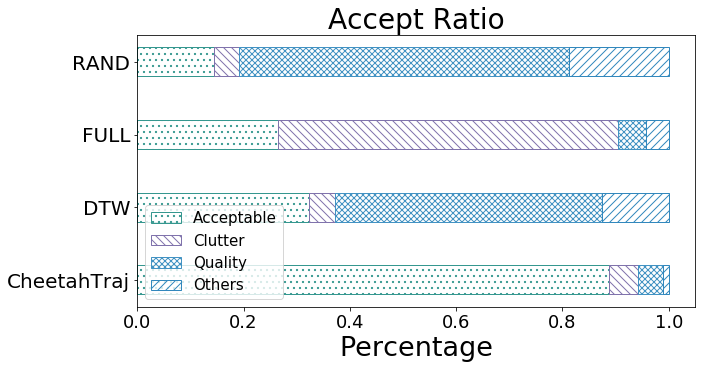
\includegraphics[width=0.35\textwidth]{pictures/user_study/accept_rate.png}
	%\vspace{-5mm}
	\caption{User study, accept rate.}
	\label{fig:accept_rate}
	%\vspace{-8mm}
\end{figure}






\subsection{Quantitative Evaluation}\label{sec:quality}
In this part, we quantitatively evaluate our proposals on the \pt{}, \cd{} and \sz{} trajectory datasets from two aspects:
(i) visual quality and (ii) running time.

\begin{figure}[t]
	\centering
	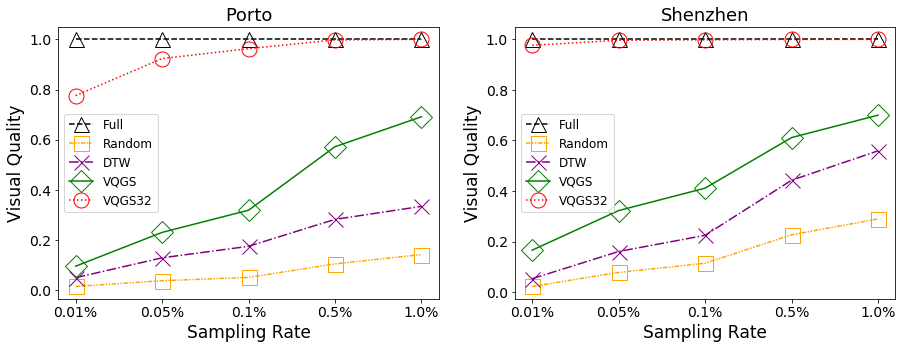
\includegraphics[width=0.5\textwidth]{pictures/quantitative_study_icde/rate_quality.png}
	\vspace{-8mm}
	\caption{Visual quality vs. sampling rates(T1).}
	\label{fig:sample_quality}
	\vspace{-3mm}
\end{figure}

\begin{figure}[t]
	\centering
	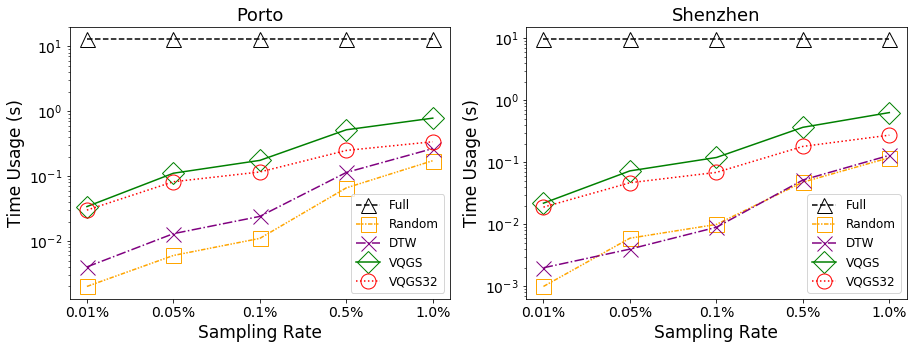
\includegraphics[width=0.5\textwidth]{pictures/quantitative_study_icde/rate_rendertime.png}
	\vspace{-8mm}
	\caption{Rendering time vs. sampling rates(T1).}
	\label{fig:rate_quality}
	\vspace{-3mm}
\end{figure}


\begin{figure}[t]
	\centering
	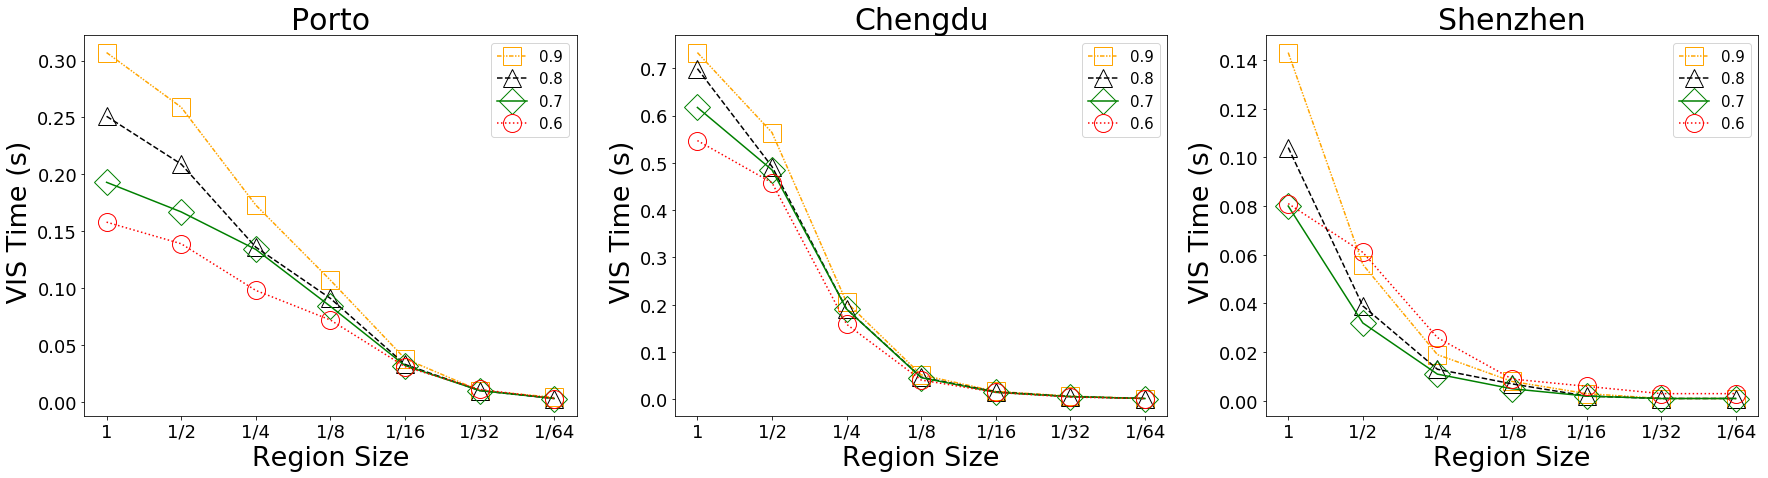
\includegraphics[width=0.5\textwidth]{pictures/quantitative_study_icde/size_rendertime.png}
	\vspace{-8mm}
	\caption{Region size vs. response time(T2).}
	\label{fig:size_rendertime}
	\vspace{-3mm}
\end{figure}

\begin{figure}[t]
	\centering
	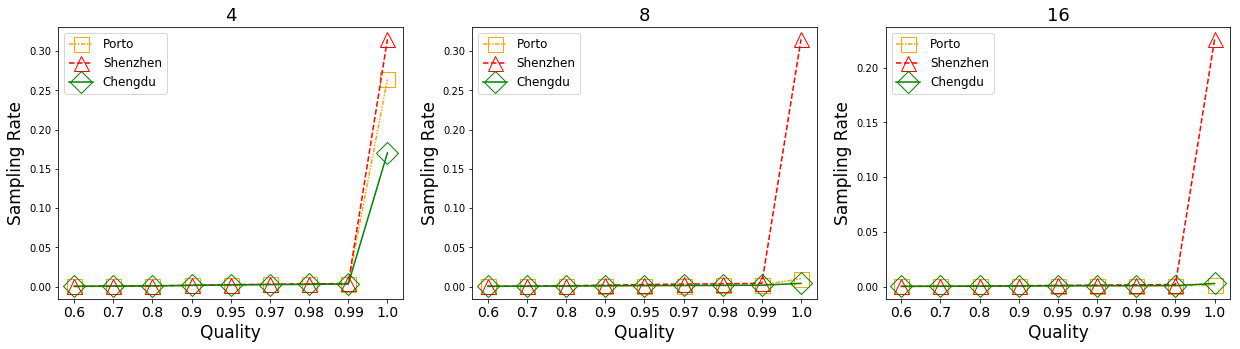
\includegraphics[width=0.5\textwidth]{pictures/quantitative_study_icde/quality_rate.png}
	\vspace{-8mm}
	\caption{Region size vs. response time(T3).}
	\label{fig:quality_rate}
	\vspace{-3mm}
\end{figure}

\begin{figure}[t]
	\centering
	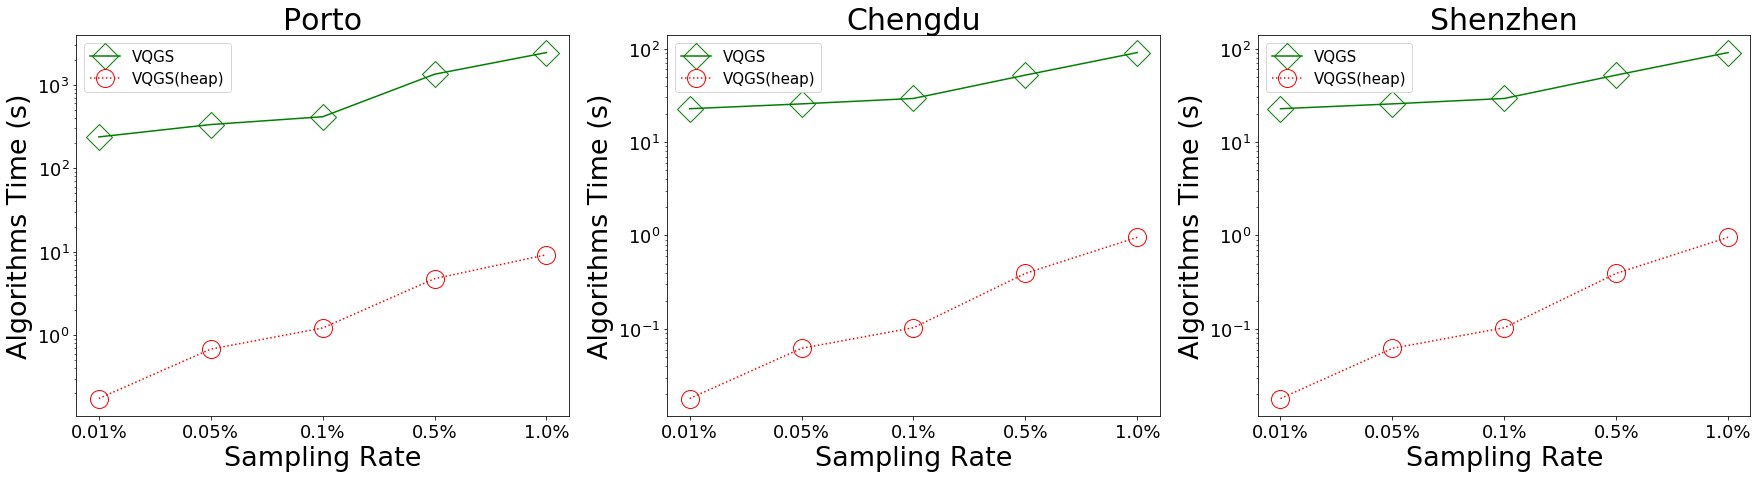
\includegraphics[width=0.5\textwidth]{pictures/quantitative_study_icde/rate_algtime.png}
	\vspace{-8mm}
	\caption{Sampling rate vs. algorithms time(T4).}
	\label{fig:rate_algtime}
	\vspace{-3mm}
\end{figure}
%\begin{figure}[t]
%	\centering
%	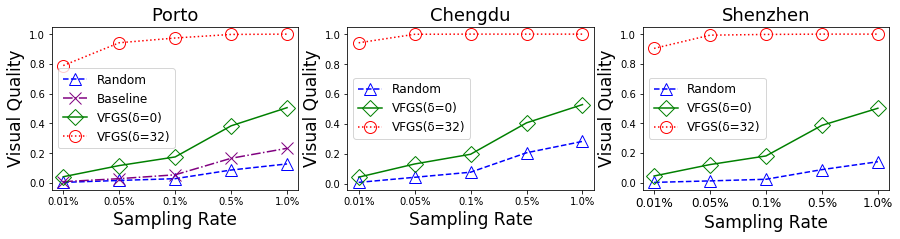
\includegraphics[width=0.5\textwidth]{pictures/quantitative_study_icde/sample_quality.png}
%	\vspace{-8mm}
%	\caption{Visual quality vs. sampling rates.}
%	\label{fig:sample_quality}
%	\vspace{-3mm}
%\end{figure}

%\begin{figure}[t]
%	\centering
%	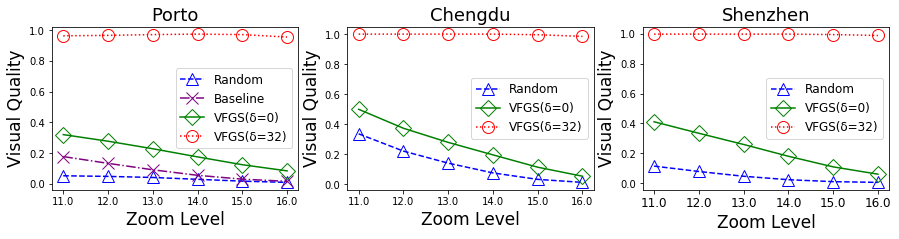
\includegraphics[width=0.5\textwidth]{pictures/quantitative_study_icde/zoom_quality.png}
%	\vspace{-8mm}
%	\caption{Visual quality vs. zoom level.}
%	\label{fig:zoom_quality}
%	\vspace{-3mm}
%\end{figure}

\stitle{Visual quality evaluation}
We evaluate the quality of proposed methods from two aspects: (i) the quality vs different zoom levels; (ii) the quality vs different sampling rates.
Visual quality is defined as the $1-loss$, in which $loss$ is the quality loss function in Equation~\eqref{eqref:loss}. The visualization using the full dataset is used as the ground-truth. 


We report the \textit{visual quality} of different visualization methods in Figure~\ref{fig:sample_quality} with a given sampling $\alpha=0.1\%$. 
The results show that $\rand$ always has the lowest visual quality. $\baseline$ is better than $\rand$ which is also confirmed by case study. Furthermore $\vats$ has better visual quality than $\baseline$ but is significantly outperformed by $\avats$. We also observed that all of the methods across the three dataset have the similar trends: the performance increases when the sampling rate increases.

Figure~\ref{fig:zoom_quality} demonstrates the relationship between visual quality and zoom level. In general, with the increase of the zoom level(zoom into the details), the visual quality drops.
We set the sampling rate $\alpha=1\%$. The results show that $\rand$ always has the lowest  visual quality. $\baseline$ performs better than $\vats$ and $\vats$ is better than $\baseline$. Moreover, $\avats$ has a much higher score than $\vats$. With $\delta=32$ , the minimum visual quality values of $\avats$ are 0.955, 0.985, and 0.989 for \pt{}, \cd{} and \sz{}, respectively. Moreover, the quality of all methods increases when the zoom level drops, which in line with Theorem~\ref{the:level}.



\stitle{Running time evaluation}

%\begin{figure}[t]
%	\centering
%	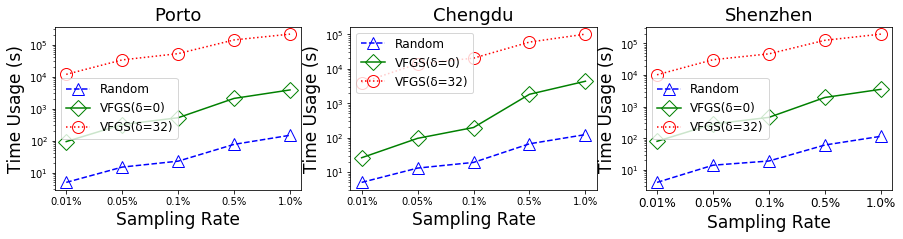
\includegraphics[width=0.5\textwidth]{pictures/quantitative_study_icde/sample_time.png}
%	\vspace{-8mm}
%	\caption{Time usage vs. sampling rates.}
%	\label{fig:sample_time}
%	\vspace{-3mm}
%\end{figure}

%\begin{figure}
%	\centering
%	\small
%	\begin{tabular}{cc}
%		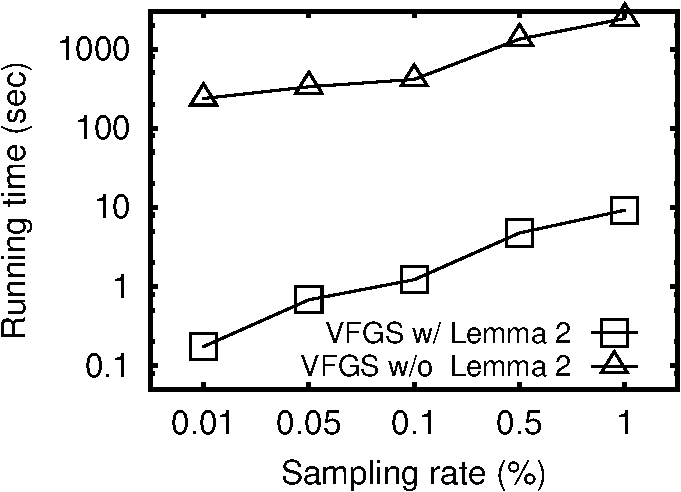
\includegraphics[width=0.44\columnwidth]{pictures/tporto}
%		&
%		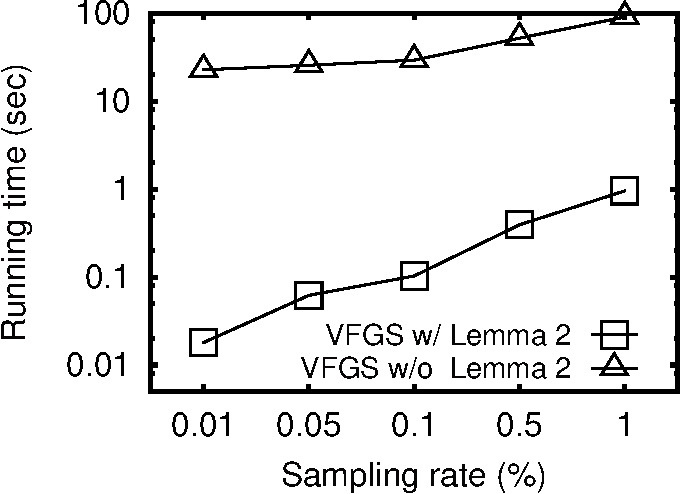
\includegraphics[width=0.44\columnwidth]{pictures/tshenzhen}
%		\\
%		(A) \pt{}
%		&
%		(B) \sz{}	
%	\end{tabular}
%	\vspace{-3mm}
%	\caption{Running time of $\vats$ w/ and w/o Lemma~\ref{lem:submodular}.}
%	\label{fig:cost}
%	\vspace{-6mm}
%\end{figure}
\QM{unfininshed}
We first conduct an experiment to evaluate the rendering cost by datasize. We vary the number of trajectories from 1000 to 1 million, which are randomly selected from \pt{} dataset. The experimental results are summarized in Table~\ref{tab:gpu}. We observe that the rendering cost is linear with the input data trajectories.

We first report the running time of our $\vats$ algorithm in Figure~\ref{fig:cost} by varying the sampling rate from $0.01\%$ to $1\%$. The results show that $\vats$ is quite slow without the submodularity of contribution value, which agrees with Lemma~\ref{lem:submodular} in Section~\ref{sec:opt}.
Then we shown the total time usage with sampling rate as Figure~\ref{fig:sample_time}. {*******}

The optimized $\vats$ (e.g., $\vats$ with Lemma~\ref{lem:submodular}) outperforms $\vats$ by one to three orders of magnitudes on both datasets. The result show that running time of our $\vats$ algorithm is below 1 second in most cases. We have shown that $\vats$ provides good visualization performance with a low sampling rate (e.g., $0.1\%$ or $1\%$) in Section 6.1 and 6.2,  and Table~\ref{tab:gpu} suggests that the rendering latency scales almost linearly with dataset cardinality. By significantly reducing the dataset cardinality with sampling, $\vats$ can effectively reduces the rendering latency to make interactive visualization possible without sacrificing visual quality. For example, rendering the full $\pt{}$ dataset takes about \QM{34 seconds}, with a sampling rate of $1\%$, $\vats$ can bring down the rendering latency to less than 1 second.

\begin{table}
	\centering
	\small
	\caption{Visualization rendering cost}
	\begin{tabular}{|c|c|c|c|c|} \hline
		No. Trajs & GPS points & Mapping (s) & Rendering (s) & Total (s)\\ \hline
		1,000& 31,300 & 0.027 & 0.003 & 0.03 \\ \hline
		10,000& 31,6531 & 0.169 & 0.005 & 0.174\\ \hline
		100,000& 316,7120 & 1.701 & 0.057 & 1.758 \\ \hline
		1,000,000& 31,646,379 & 15.562 & 0.592 & 16.154 \\ \hline
	\end{tabular}	\label{tab:gpu}
\end{table}



\section{Conclusions and future directions}\label{sec:con}
%Visualizing large trajectory dataset is challenge due to two reasons: visual clutter and long rendering time.
%Data sampling technique, an effective method in reducing the rendering time by shrinking the data size, has been applied in a variety of data.
%However, very few work target at the trajectory sampling especially from the perspective of visualization.
%The most commonly used sampling method, uniform random sampling technique, always generate results with very poor visual quality because very few trajectories located at margin regions can be preserved.
%We fill the gap by proposing a novel sampling techniques $\avats$ which guarantees the visual quality at overview and reduce the visual clutter at the detail view. The technique characteristics and a series of parameters setting are discussed.
%We compare $\avats$ with uniform random sampling in regarding to visual quality preservation and time-usage. We evaluate the effectiveness of proposed method by applying our method to different dataset and conducting users studies on specific interactive trajectory exploration tasks.
%Even though it is recommended to use our method with caching techniques, our experience in the experiment shows that a faster algorithm will be more user friendly for the real world ad-hoc exploration tasks. For future work, we first plan to reduce the time usage by leveraging the advanced database techniques such as the indexing technique or use GPU acceleration.
%In addition, there are several directions can be further explored to enrich the information presented by the visualization.
%First we will develop different color encoding schema to present the spatial distribution of trajectory more precisely.
%In current schema, the color of one trajectory is the same, thus the color of the long trajectories may mislead the users because they pass  through many regions with different level of the traffic crowdedness. One solution is to use gradient color schema to encode the trajectories.
%Another interesting direction is to extend the approach to support the mulit-class characteristics which is a commonly existed in variety of trajectory dataset.
This paper presents a novel sampling technique, $\avats$, that guarantees the visual quality of line-based trajectory visualization and alleviates the visual clutter problem. The effectiveness and efficiency of the proposed method are validated with real world visual analysis tasks and quantitatively performance measurements. Possible future directions include (i) improving visual quality by sampling trajectory segments instead of complete trajectories and (ii) developing advanced color encoding schemes to better describe the spatial distribution of the trajectories.
%extending our approaches to support the specific trajectory features such as mulit-class characteristics.

%we focus on the sampling approach of trajectory segments other than the whole trajectories to achieve higher visual fidelity.
%We will also develop different color encoding schema to present the spatial distribution of trajectories more precisely. Currently, the color of one trajectory keep the same, thus the color of the long trajectories may mislead the users because they may pass through many regions with different traffic crowdedness.
%We also consider to extend our approach to support the specific trajectory features such as mulit-class characteristics. 


\bibliographystyle{IEEEtran}
\bibliography{ref}

\end{document}
